\title{継続的インテグレーションを用いた文書検査システムの構築}
\author{プロジェクトマネジメントコース\\
ソフトウェア開発管理グループ\\
矢吹研究室\\
1342097\\
浜野 太豪}
\date{}
\begin{document}
\maketitle

%本テンプレートの余白は,卒論マニュアルで指示されたものとは違っているが,1ページあたりの文字数は40文字x40行と,卒論マニュアル通りになっている。文字間隔や行間隔を調整して,余白をマニュアル通りにすることもできるが,それでは文章が読みにくくなるため,このような対応をしている。

%\noindent
□□□□□□□□□■□□□□□□□□□■□□□□□□□□□■□□□□□□□□□■
□□□□□□□□□■□□□□□□□□□■□□□□□□□□□■□□□□□□□□□■
□□□□□□□□□■□□□□□□□□□■□□□□□□□□□■□□□□□□□□□■
□□□□□□□□□■□□□□□□□□□■□□□□□□□□□■□□□□□□□□□■
□□□□□□□□□■□□□□□□□□□■□□□□□□□□□■□□□□□□□□□■
□□□□□□□□□■□□□□□□□□□■□□□□□□□□□■□□□□□□□□□■
□□□□□□□□□■□□□□□□□□□■□□□□□□□□□■□□□□□□□□□■
□□□□□□□□□■□□□□□□□□□■□□□□□□□□□■□□□□□□□□□■
□□□□□□□□□■□□□□□□□□□■□□□□□□□□□■□□□□□□□□□■
□□□□□□□□□■□□□□□□□□□■□□□□□□□□□■□□□□□□□□□■
□□□□□□□□□■□□□□□□□□□■□□□□□□□□□■□□□□□□□□□■
□□□□□□□□□■□□□□□□□□□■□□□□□□□□□■□□□□□□□□□■
□□□□□□□□□■□□□□□□□□□■□□□□□□□□□■□□□□□□□□□■
□□□□□□□□□■□□□□□□□□□■□□□□□□□□□■□□□□□□□□□■
□□□□□□□□□■□□□□□□□□□■□□□□□□□□□■□□□□□□□□□■
□□□□□□□□□■□□□□□□□□□■□□□□□□□□□■□□□□□□□□□■
□□□□□□□□□■□□□□□□□□□■□□□□□□□□□■□□□□□□□□□■
□□□□□□□□□■□□□□□□□□□■□□□□□□□□□■□□□□□□□□□■
□□□□□□□□□■□□□□□□□□□■□□□□□□□□□■□□□□□□□□□■
□□□□□□□□□■□□□□□□□□□■□□□□□□□□□■□□□□□□□□□■
□□□□□□□□□■□□□□□□□□□■□□□□□□□□□■□□□□□□□□□■
□□□□□□□□□■□□□□□□□□□■□□□□□□□□□■□□□□□□□□□■
□□□□□□□□□■□□□□□□□□□■□□□□□□□□□■□□□□□□□□□■
□□□□□□□□□■□□□□□□□□□■□□□□□□□□□■□□□□□□□□□■
□□□□□□□□□■□□□□□□□□□■□□□□□□□□□■□□□□□□□□□■
□□□□□□□□□■□□□□□□□□□■□□□□□□□□□■□□□□□□□□□■
□□□□□□□□□■□□□□□□□□□■□□□□□□□□□■□□□□□□□□□■
□□□□□□□□□■□□□□□□□□□■□□□□□□□□□■□□□□□□□□□■
□□□□□□□□□■□□□□□□□□□■□□□□□□□□□■□□□□□□□□□■
□□□□□□□□□■□□□□□□□□□■□□□□□□□□□■□□□□□□□□□■
□□□□□□□□□■□□□□□□□□□■□□□□□□□□□■□□□□□□□□□■
□□□□□□□□□■□□□□□□□□□■□□□□□□□□□■□□□□□□□□□■
□□□□□□□□□■□□□□□□□□□■□□□□□□□□□■□□□□□□□□□■
□□□□□□□□□■□□□□□□□□□■□□□□□□□□□■□□□□□□□□□■
□□□□□□□□□■□□□□□□□□□■□□□□□□□□□■□□□□□□□□□■
□□□□□□□□□■□□□□□□□□□■□□□□□□□□□■□□□□□□□□□■
□□□□□□□□□■□□□□□□□□□■□□□□□□□□□■□□□□□□□□□■
□□□□□□□□□■□□□□□□□□□■□□□□□□□□□■□□□□□□□□□■
□□□□□□□□□■□□□□□□□□□■□□□□□□□□□■□□□□□□□□□■
■■■■■■■■■■■■■■■■■■■■■■■■■■■■■■■■■■■■■■■■
□□□□□□□□□■□□□□□□□□□■□□□□□□□□□■□□□□□□□□□■%文字数チェック用

\chapter*{謝辞}

本研究を進めるにあたり,矢吹研究室矢吹太朗准教授には,多くの時間をご指導にさいて頂きました.
また矢吹研究室の皆様には,多くの知識や示唆を頂きました.協力していただい皆様に感謝の気持ちと御礼を申し上げます.

\tableofcontents%目次


\chapter{序論}
ドキュメントの検査にプログラムやツールによるサポートが必要である.なぜなら,システム開発の現場では,様々なドキュメントを作成する必要があるからだ.例えばプロジェクト計画書や要件定義書,マニュアルなどがある.このような文書では,読み手に誤解を与えてはいけない.さらに,わかりやすい文書を書くには一定のルールを守る必要がある.短い文で書くこと,正しい表現方法で書くこと,フォーマットを統一することなどである.このようなルールで,大量のドキュメントを人の目によってチェックすることには限界がある.

そこで継続的インテグレーションを活用する方法がある.継続的インテグレーションとは,プログラム全体を常に統合して動く状態にしておくことである.最近では,ビルド(プログラムのコンパイルや自動テスト,アーカイブ化,ソースコードへのタグ付け,実行環境へのデプロイの一連の手順)を自動化するツールが数多くある\cite{5}.

このような継続的インテグレーションで活用されている自動化ツールを用いて,大量のドキュメントをチェックできるツールを構築する.









\chapter{目的}
文書チェックを自動的に行うシステムを構築する.
研究室ではドキュメントの変更履歴をバージョン管理システムGitHubを用いて管理している.GitHubに文書を提出した際に,自動で文書チェックプログラムが実行され,実行結果の表示,通知を行う.


\chapter{利用するサービスの解説}
本研究では継続的インテグレーションを用い,文書の自動検査を行う.継続的インテグレーションを行うツールとしてWercker,ビルド環境の構築にDocker,文書検査のビルドにRedpenというサービスを用いる.
以下のサービスの解説を行う.


\section{RedPen}
\begin{figure}[htb]
\centering 
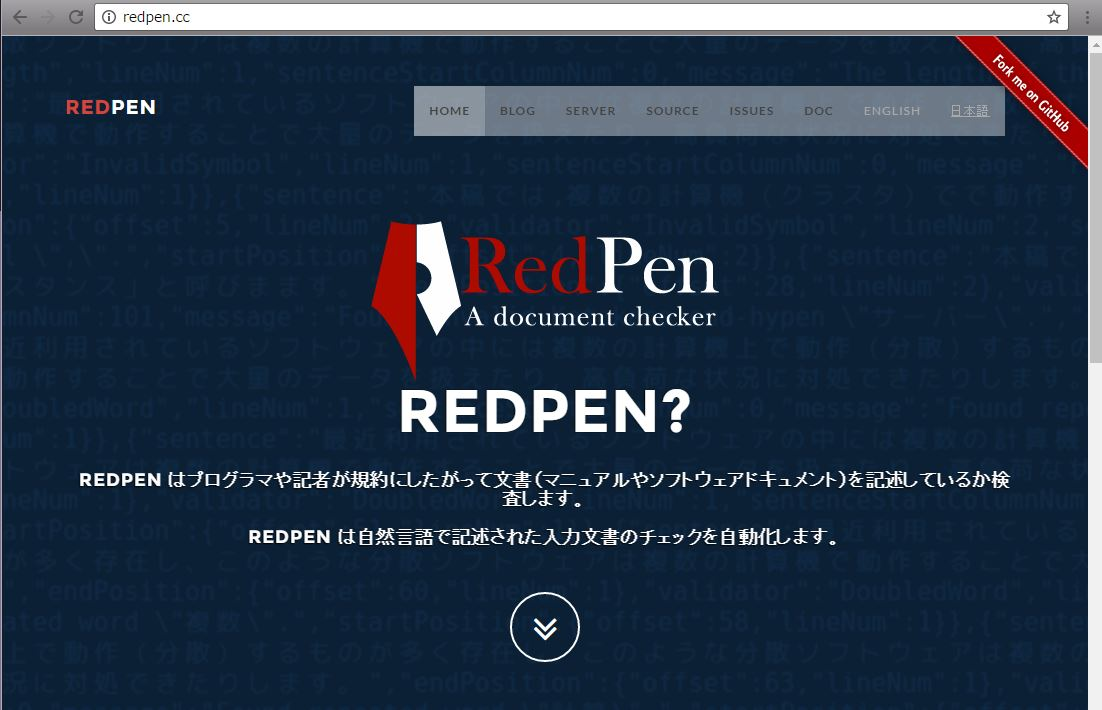
\includegraphics[width=11cm]{28.JPG}
\caption{RedPen}\label{tab:uac}
\end{figure}
RedPenは技術文書をターゲットにした文書の自動検査ツールである.技術文書にはマニュアルやチュートリアル,論文,仕様書等が含まれる.
技術文書にはわかりやすさが求められる.詩や歌謡曲の歌詞にはわかりやすさを放棄し,わざと曖昧な部分を残すことでより心に響く作品となる場合がある.しかしわかりやすさが第一に求められる技術文書には余韻や深みは必要ない.

日記等と違って技術文書は自分以外の第三者が読むため,恥ずかしくない文書を書く必要がある.恥ずかしい文書は利用する特殊文字や専門用語が揃っていなかったり,"彼がが行く" のように明らかな文法間違いが多数存在する.また"すごい"や"っていうか"などの口語が混じってしまっていると,文書のみならず,文書が扱う製品の品質までにあらぬ疑いをもたれてしまう.

RedPenは技術文書を書く上の規約にしたがって文書を記述しているか検査するツールである.

そのほかにRedPenの特徴として柔軟な設定,言語非依存,マークアップ言語サポートがあげられる.
柔軟な設定ではRedPenの設定ファイルを変更することで検査仕様の変更が容易に行える.言語非依存ではどのような言語で書かれた文書でも処理することができる.もちろん日本語に対応している.マークアップ言語サポートでは多様なフォーマット(Markdown,LaTeXなど)で記述された文書をそのまま検査できる\cite{1}.


\newpage
\section{Github}
\subsection{Git}
Git(ギット)とは,2005年に開発された,ファイルやプログラミングコード,文書の変更履歴を管理するためバージョン管理ツールのことである.

\begin{figure}[htb]
\centering 
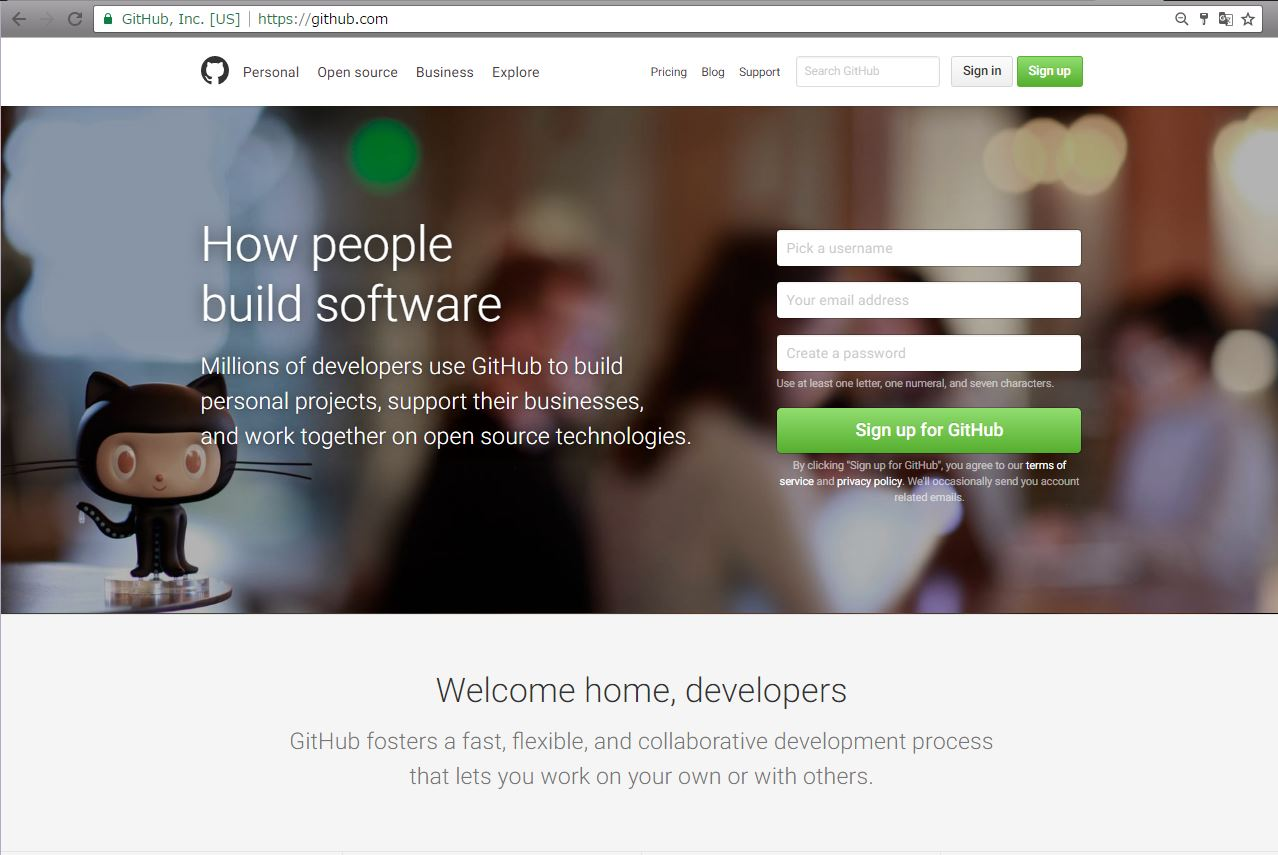
\includegraphics[width=11cm]{29.JPG}
\caption{GitHub}\label{tab:uac}
\end{figure}
GitHubは2008年オープンした,Gitのリモートリポジトリと,さまざまなWebツールを提供するサービスである.オープンソースソフトウェアは,時間的にも地理的にも離れたところに住む複数のプログラマによって開発される.GitHubでは相談して課題を解決するIssue(イシュー)や改善案を気軽に提案できるPull Request(プルリクエスト)などの機能が,注目を集めている.\cite{2}
 GitHubのさまざまな機能を一部抜粋して,説明を記述する.



\subsection{リポジトリ}

ファイルやディレクトリの状態を記録する場所.

\subsection{リモートリポジトリ}

手元に置いてあるローカルなリポジトリ以外の,ネット上に置かれたリポジトリのこと.

\subsection{commit}

ファイルやディレクトリの変更をリポジトリに記録する機能である.


\subsection{clone}

ネット上にあるリポジトリをローカルにコピーする機能である.


\subsection{Origin}

clone元のリモートリポジトリのこと.


\subsection{Push}

リモートリポジトリに自分の変更履歴がアップロードされ,リモートリポジトリ内の変更履歴がローカルリポジトリの変更履歴と同じ状態にする機能である.


\subsection{branch}

履歴の流れを分岐して記録していくためのもの.分岐したブランチは,他のブランチの影響を受けないため,同じリポジトリ中で複数の変更を同時に進めていける機能である.


\subsection{pull}

リモートリポジトリから最新の変更履歴をダウンロードしてきて,自分のローカルリポジトリにその内容を取り込む機能である.


\subsection{Pull Request}

相手に対して自分の変更ををpullしてもらうように要求する機能である.


\subsection{Revert}

ステージングエリアに追加した変更を取り消す機能である.

\subsection{タグ}

コミットを参照しやすくするために,わかりやすい名前を付ける機能である.


\subsection{Label}

自由に作成でき,Issueをフィルタリングできる機能である.


\subsection{Merge}

当該ブランチに対して別のブランチの差分を取り込むことである.


\subsection{Fork}

GitHubのサービスで,相手のリポジトリを自分のリポジトリとしてコピー・保持できる機能ある.


\subsection{Issue}

ソフトウェア開発におけるバグや議論などをトラッキングして管理するために発行する.

\subsection{デプロイ}

ソフトウェアの分野で,開発したソフトウェアを利用できるように実際の運用環境に展開する.


\subsection{リリース}

プロセスを次の段階に進めることを認める機能である.


\subsection{Watch}

リポジトリに関する情報をNotificationsに表示する機能である.

\subsection{Star}

リスト一覧からリポジトリを探すことが出来るようにする機能である.
また,注目度を表す指標にもなる.

\subsection{Fork}

GitHub側にある特定のリポジトリを自分のアカウント以下のリポジトリに複製する機能である.

\subsection{人数}
開発人数のことである.
ここでは,Originリポジトリにコミットした人数のことを示す.

\subsection{MileStone}

やるべきタスクの管理にIssueを用いることができるようにする機能である.

\subsection{Wiki}

簡単な記法によってドキュメントを作成,編集するための機能である.

\newpage
\section{Wercker}
\begin{figure}[htb]
\centering 
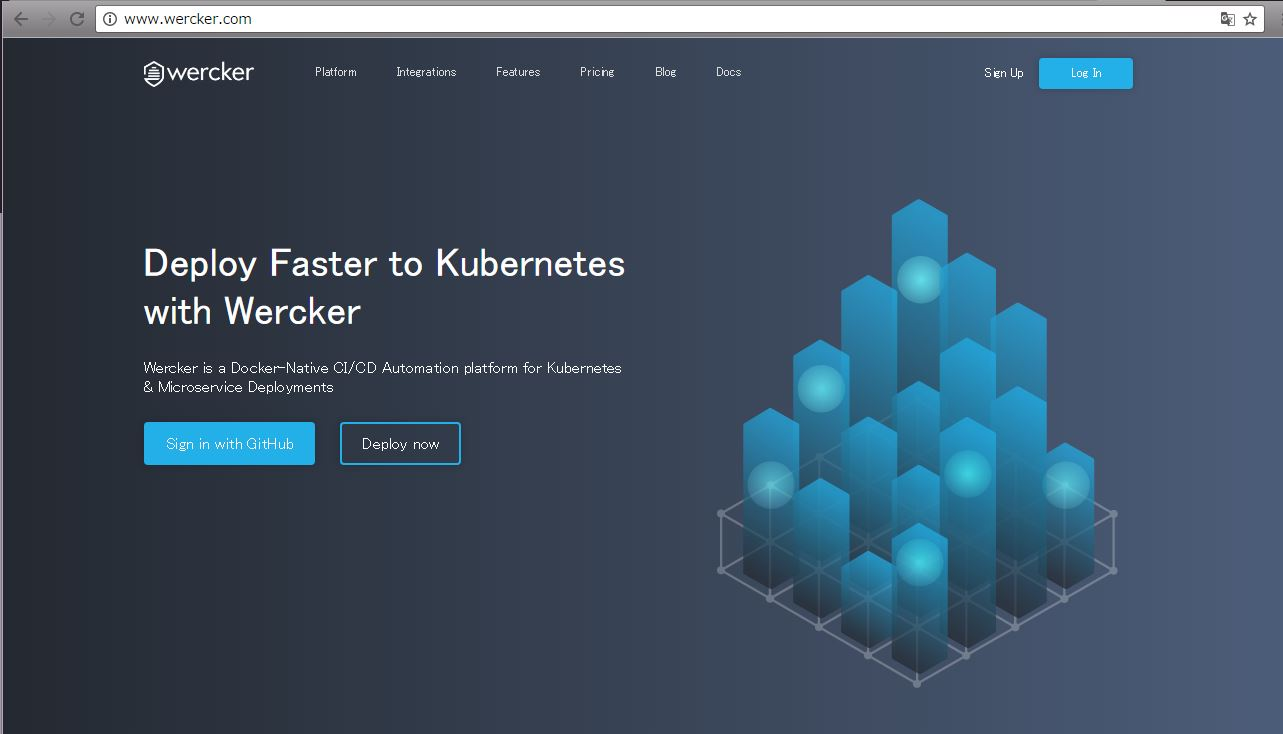
\includegraphics[width=11cm]{30.JPG}
\caption{Wercker}\label{tab:uac}
\end{figure}
WerckerとはGitHubにコードをプッシュすれば自動的にアプリのテスト・ビルドデプロイを行うことができるCI(継続的インテグレーション)サービスである.
WerckerはGitHubのリポジトリにwercker.ymlを準備そこに記述された実行環境と続行コマンドをもとにテスト/ビルドを走らせる.

\newpage

以下にサンプルのwercker.ymlファイルを示す.
\begin{lstlisting}[basicstyle=\ttfamily\footnotesize, frame=single]
box: wercker/ruby
services:
    - mies/rethinkdb
build:
    steps:
        # Execute the bundle install step, a step provided by wercker
        - bundle-install
        # Execute a custom script step.
        - script:
            name: middleman build
            code: bundle exec middleman build --verbose
deploy:
    steps:
        # Execute the heroku-deploy, heroku details can be edited
        # online at http://app.wercker.com/
        #- heroku-deploy

        # Execute the s3sync deploy step, a step provided by wercker
        - s3sync:
            key_id: $AWS_ACCESS_KEY_ID
            key_secret: $AWS_SECRET_ACCESS_KEY
            bucket_url: $AWS_BUCKET_URL
            source_dir: build/
    after-steps:
        - hipchat-notify:
            token: $HIPCHAT_TOKEN
            room-id: id
            from-name: name
\end{lstlisting}

上からbox,services,buildフェーズ,deployフェーズ,stepを記述していく.
boxはOSと一連のパッケージがインストールされたVMである.例えばrubyがインストールされたbox,Golangがインストールされたboxなどがある.
boxはWerckerが提供するもの,もしくはDockerで構築したものを利用することができる.

\newpage

\section{Docker}
\begin{figure}[htb]
\centering
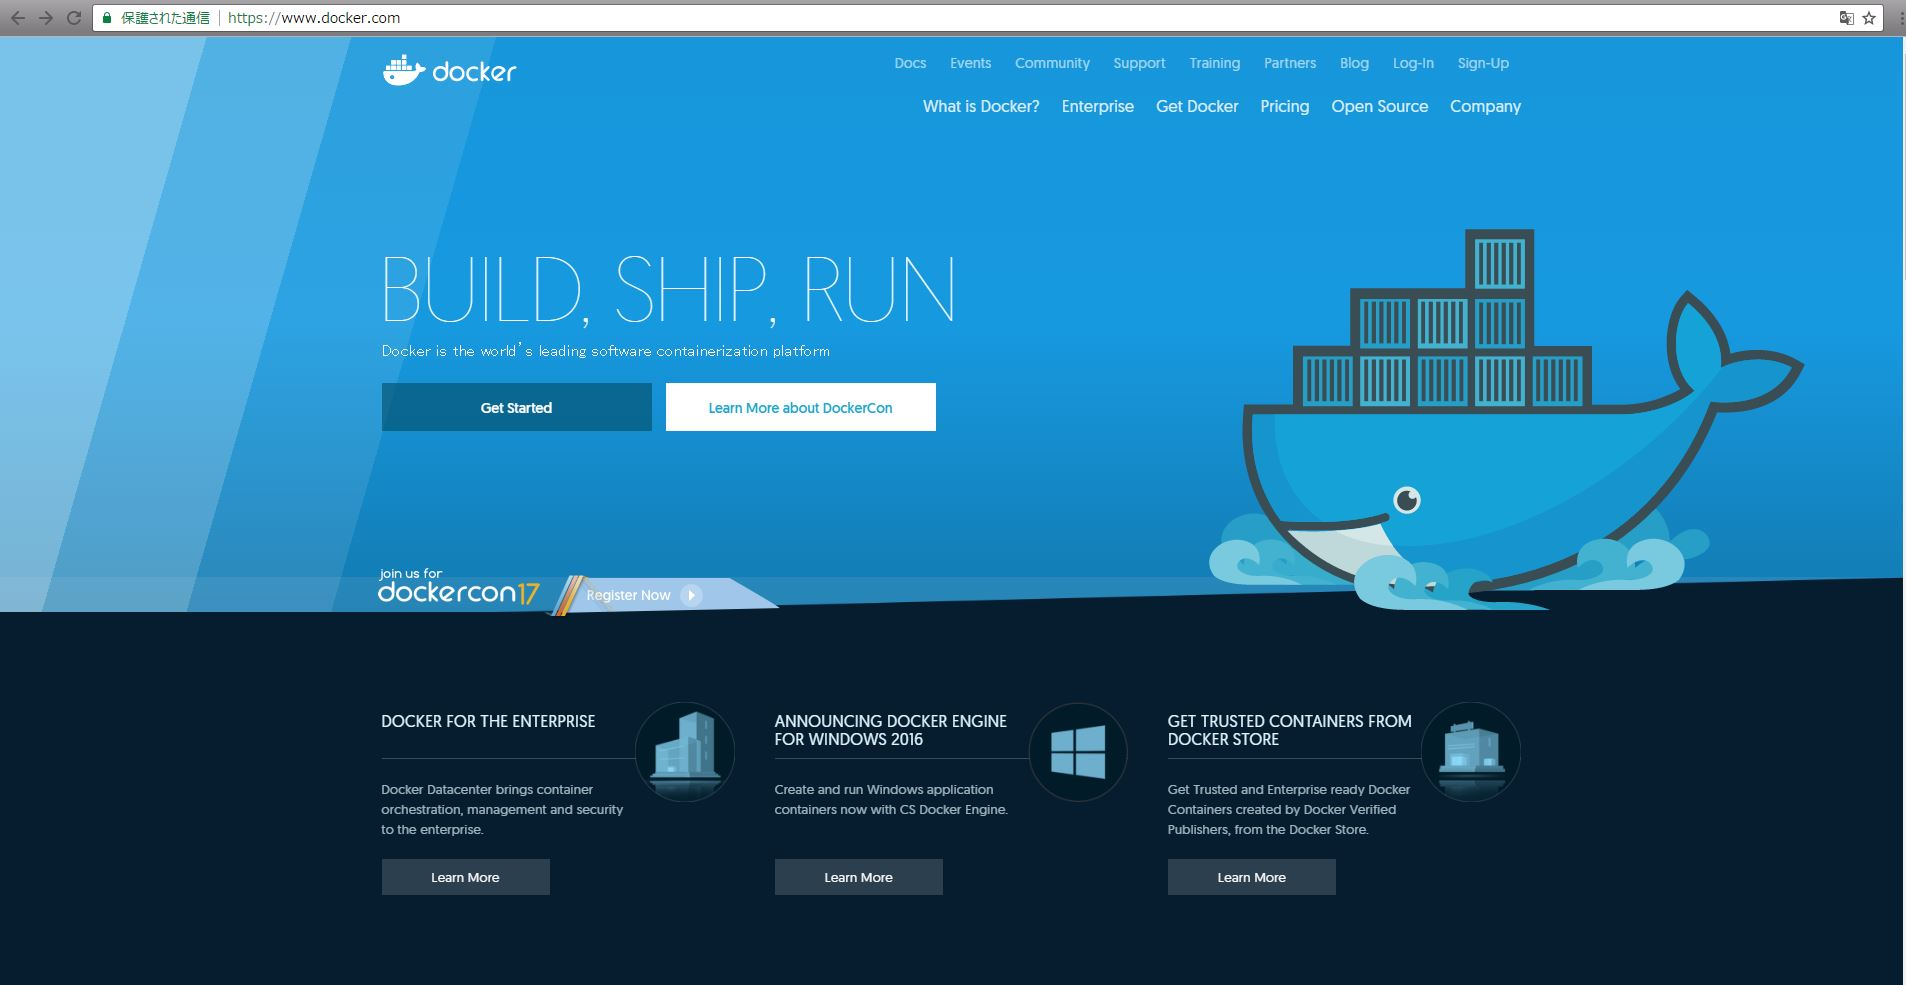
\includegraphics[width=11cm]{33.JPG}
\caption{Dockerホームページ}\label{tab:uac}
\end{figure}
Dockerとは,Linuxのコンテナ技術をベースにDocker社が開発した仮想化技術である.アプリ実行環境を高速にデプロイできるコンテナ型の仮想化マシンである\cite{3}.
WindowsOSの内部に独立したアプリケーションの実行環境であるコンテナを生成することができ,リソース消費量が非常に少なく1台の物理サーバに多くのコンテナを稼働させられる.

\newpage

\subsection{DockerHubのアカウント登録}
複数のマシンで共通の環境を共有するために,作成した環境であるコンテナをDockerHubにアップロードし公開することができる.

DockerHubのアカウント登録は以下を参照する.
https://hub.docker.com/
\begin{figure}[htb]
\centering
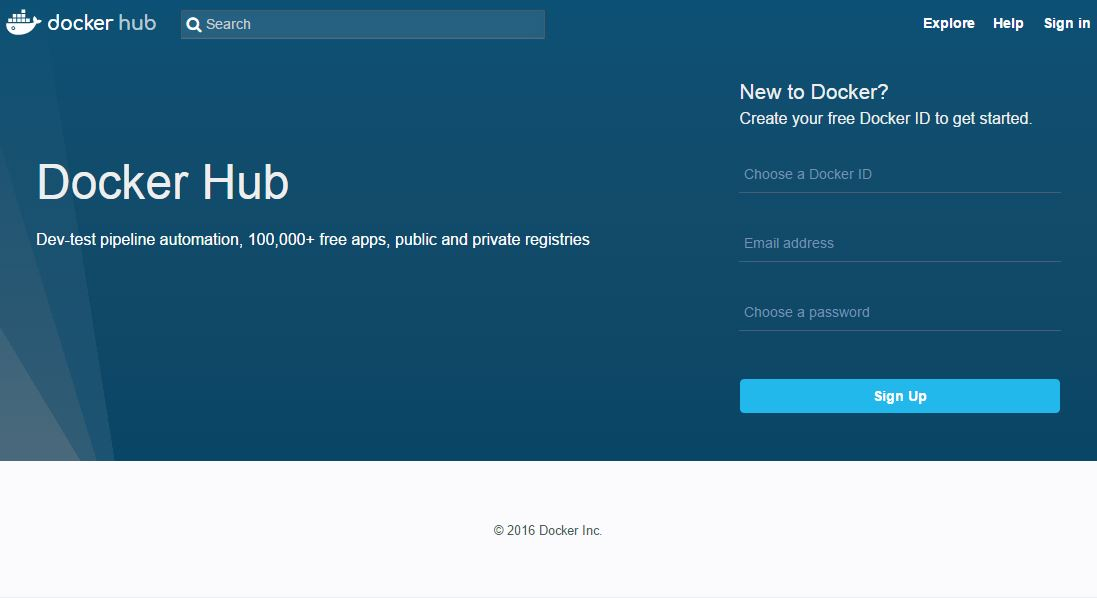
\includegraphics[width=11cm]{26.JPG}
\caption{DockerHubホームページ}\label{tab:uac}
\end{figure}

\chapter{開発環境構築ツールの解説}

\section{Chocolatey}
\begin{figure}[htb]
\centering
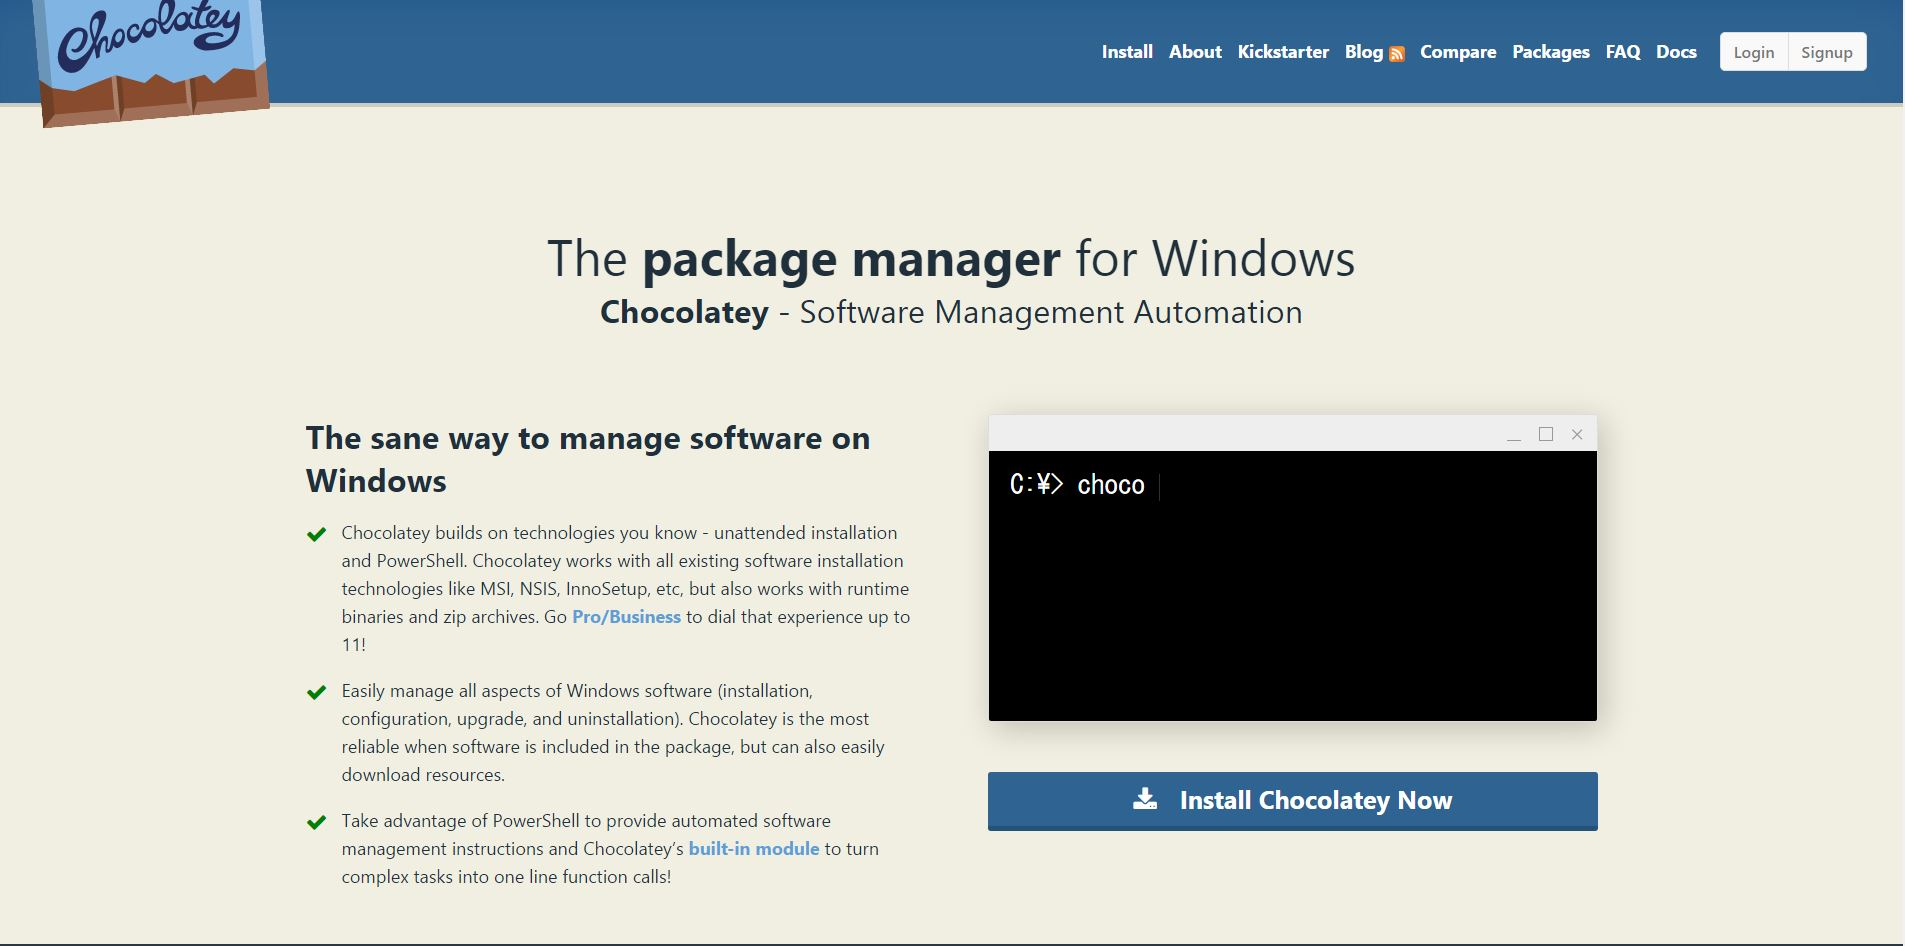
\includegraphics[width=11cm]{32.JPG}
\caption{chocolatey}\label{tab:uac}
\end{figure}
「Chocolatey」は,コマンドラインによるアプリケーションの導入や削除を実現するパッケージ管理システム.パッケージ管理システムとは,アプリケーションやコンポーネント,ライブラリなどの管理を円滑に行うための仕組み.アプリケーションやライブラリを構成するファイル群を1つの”パッケージ”ファイルにまとめ,それを”リポジトリ”へ保管し,コマンドで取得・セットアップを行う.動作に必要な外部コンポーネントがあれば,その導入も自動で行われるのが一般的で,アプリケーションのインストールやアンインストールの手間を省くことができる.

Linuxディストリビューションの多くは”apt-get”や”yum”といったパッケージ管理のためのコマンドを備えており,コマンドを入力するだけで手軽にソフトをダウンロード・インストール・アンインストールできて非常に便利.「Chocolatey」はこれをWindows環境で実現しようというものである.



\subsection{パッケージとは}
ソフトウェアにかかわるファイル一式がまとまったものをパッケージという.「ソフトウェアにかかわるファイル」には,設定ファイルやドキュメント,プログラム本体,プログラムが動くために必要なライブラリなどが含まれます.

\subsection{choco list [packageName]}
 パッケージ検索.引数がなければすべてのパッケージを表示.
\subsection{choco list -lo [packageName] }
インストール済みのパッケージ検索.引数がなければすべてのインストール済みパッケージを表示.
\subsection{cinst [packageName]}
 指定パッケージのインストール.
\subsection{cuninst [packageName]}
 指定パッケージのアンインストール.
\subsection{cup}
 Chocolatey本体のアップデート.
\subsection{cup [packageName]}
 指定パッケージのアップデート.
\subsection{cup all}
 インストール済みのパッケージを全てアップデート.

\newpage
\section{DockerToolBox}
Docker Toolboxは,Docker環境を簡単に構築するためのインストーラである.現在,MacとWindows用に提供されている.

Dockerは,Linux上で動作するため,Windowsでは,Dockerを動作させるためLinux仮想マシンを用意し,それを利用する形態をとる.

Docker Toolboxは,このDocker環境を構築・運用するためのアプリケーションやツールをセットにして提供する.
Docker Toolboxのセット内容は,以下のとおりである.
\begin{table}[htb]
    \begin{center}
         \caption{仮想マシンの操作}
            \begin{tabular}{|l|c|r||r|} \hline
                ツール & 概要  \\ \hline \hline
                Docker Client & Dockerを操作するツール(dockerコマンド)  \\ \hline
                Docker Machine & Docker仮想マシンを簡単に構築・管理するためのツール  \\ \hline
                Docker Compose & マルチコンテナアプリケーション(複数のコンテナで構成するシステム)  \\ \hline
                Docker Kitematic & DockerをGUIで操作するツール  \\ \hline
                Docker Quickstart Terminal & dockerコマンドが即利用できるターミナル \\ \hline
                VirtualBox & PCの仮想化アプリケーション  \\ \hline
                \end{tabular}
     \end{center}
\end{table}


\newpage

\section{Oracle VM VirtualBox}
Oracle VM VirtualBox(以下,VirtualBoxと表記する)は,使用しているPCマシン上に仮想的なマシンを作成し,別のOSをインストール・実行することができるオープンソースソフトウェアである.WindowsやMac OS X,Linux等,様々なOSで利用することができる
本研究で利用するVirtualBoxの用語について説明する.
\subsection{ホストPC}
VirtualBoxをインストールしたPCのこと.

\subsection{ホストOS}
VirtualBoxをインストールしたPCのOSのこと.本研究で使用するホストPCのOSはWindows 7/8.1である. 

\subsection{ゲストPC(仮想マシン)}
VirtualBoxで作成した仮想PC

\subsection{ゲストOS}
VirtualBoxで作成した仮想PCにインストールしたOSのこと.










\chapter{開発環境の導入}

パッケージ管理システム「Chocolatey」をインストールするためには、管理者権限でコマンドプロンプトを起動する必要がある.Windows 10の場合,「スタート」ボタンを右クリックして,「コマンドプロンプト(管理者)」をクリックする.
\begin{figure}[htb]
\centering 
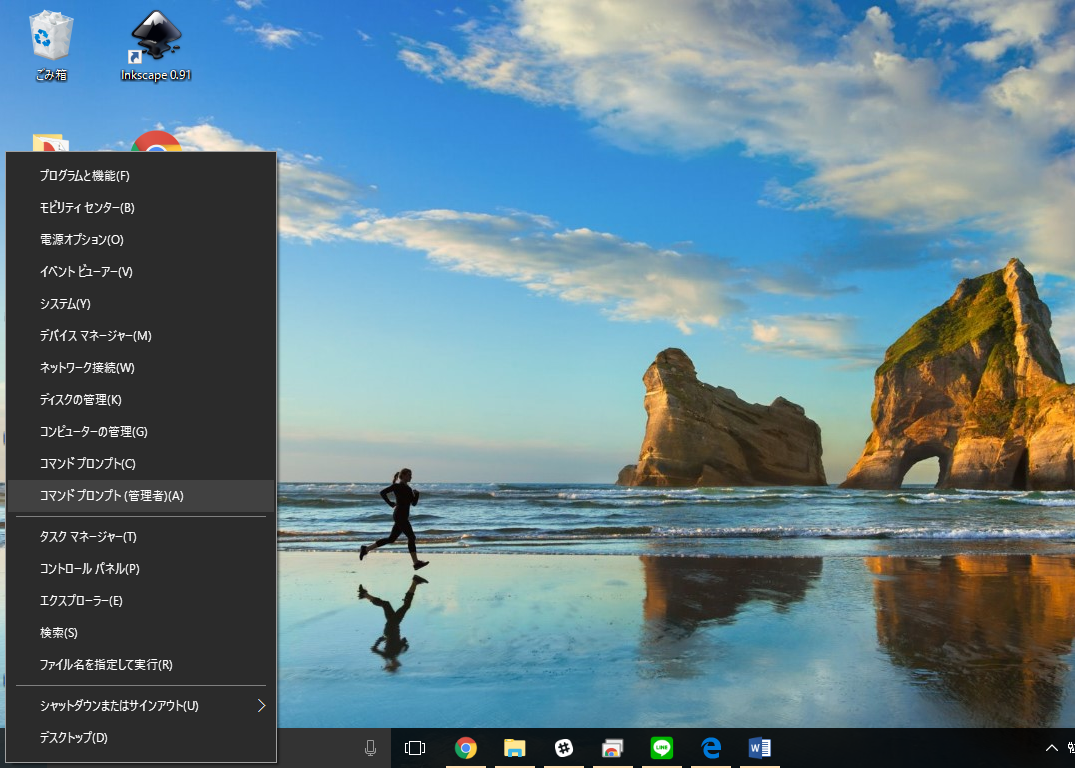
\includegraphics[width=11cm]{desktop.png}
\caption{管理者権限}\label{tab:desktop}
\end{figure}


\begin{figure}[htb]
\centering 
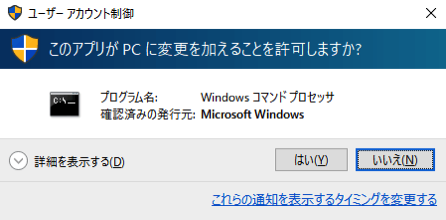
\includegraphics[width=11cm]{uac.png}
\caption{UAC}\label{tab:uac}
\end{figure}
\newpage

UAC(User Account Control)が有効になっている場合は,コマンドプロンプトを管理者権限で実行して良いかどうかプロンプトが表示されるため,「はい」をクリックする.



hocolatey」をインストールするために、コマンドプロンプトで、以下のコマンドを実行する.

\begin{lstlisting}[basicstyle=\ttfamily\footnotesize, frame=single]
@powershell -NoProfile -ExecutionPolicy Bypass -Command "iex ((Ne
w-Object System.Net.WebClient).DownloadString('https://chocolatey.org
/install.ps1'))" && SET "PATH=%PATH%;%ALLUSERSPROFILE%\chocola
tey\bin"
\end{lstlisting}

\newpage

\begin{figure}[htb]
\centering 
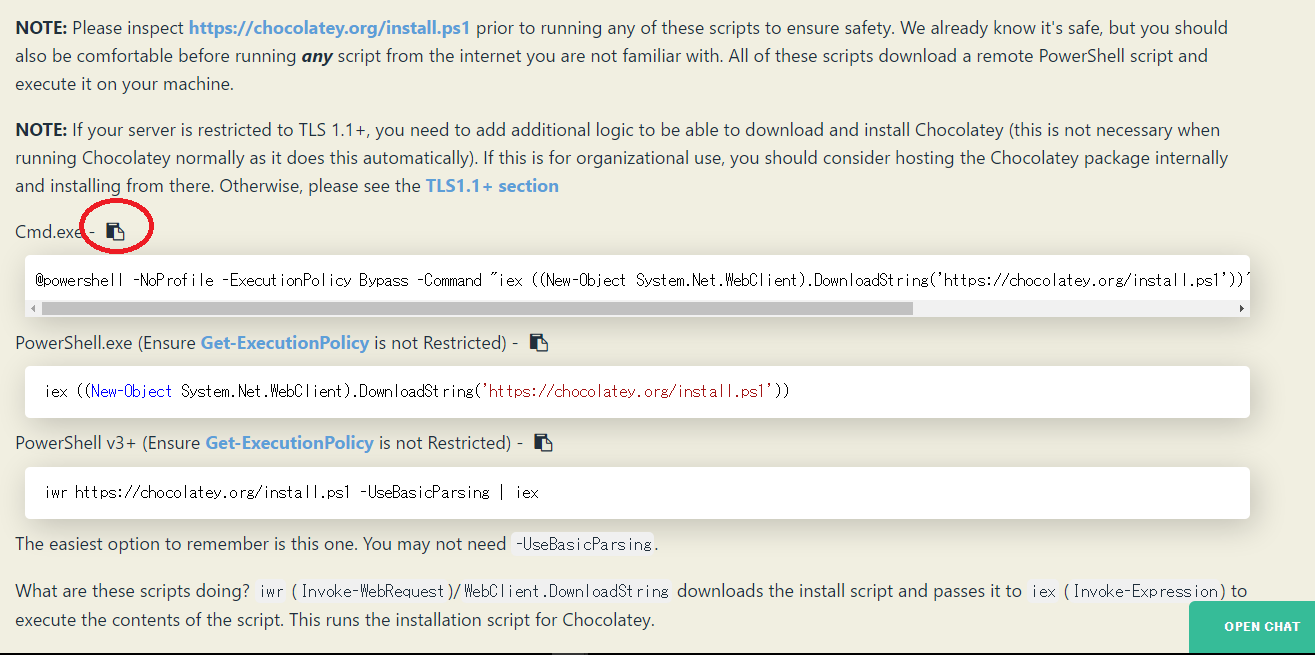
\includegraphics[width=11cm]{choco2.png}
\caption{chocoインストール}\label{tab:uac}
\end{figure}


インストール方法は,今後変更される可能性がある.そのため,以下のコマンドが正常に動作しない場合は,Chocolatey Galleryから最新の情報を確認してください.

\newpage

\subsection{パッケージのインストール}
「VirtualBox」と「vagrant」,「WinSCP」をChocolateyを使って,コマンドプロンプトからインストールする.
「VirtualBox」と「vagrant」,「WinSCP」をインストールするために,コマンドプロンプトで,以下のコマンドを実行する.



\begin{lstlisting}[basicstyle=\ttfamily\footnotesize, frame=single]
$ cinst -y atom chrome curl git github r.project rsync sourcetree vagrant 
virtualbox wget
\end{lstlisting}
\newpage


\section{Dockerのインストール}
DockerはLinuc上でコンテナ仮想環境を構築するツールである.これをWindows環境で実行するには,まずWindows上に仮想環境を構築し,そこでLinuxサーバを動作させる必要がある.

Docker ToolBoxをインストールすれば,Windows上にVirtualBoxによる仮想環境を構築し,Docker用の仮想マシンイメージを起動し,その上でDockerを稼働させる環境を構築できるcite{4}.



インストールを行うにはPCのBIOS設定でCPUの仮想化支援機能を有効にしておく必要があります.たとえば,仮想化支援機能を有効にすると,タスクマネージャの「パフォーマンス」タブの「CPU」で「仮想化」が有効になっています.設定が有効でない場合は,CPUの仮想化支援機能を有効にしてください.

\begin{figure}[htb]
\centering 
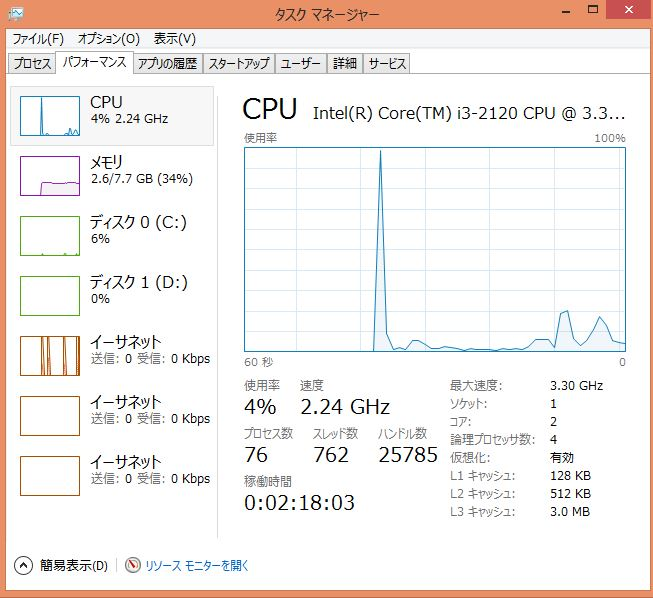
\includegraphics[width=11cm]{1.JPG}
\caption{タスクマネージャの「パフォーマンス」タブ}\label{tab:uac}
\end{figure}
BIOS設定画面はWindowsの場合,起動中の画面で「F2」キーまたは「Delete」キーを押すと,BIOS画面が表示されます.
\newpage

\subsection{Docker Toolboxのダウンロードとインストール}
Docker Toolboxのダウンロードは以下のサイトからできる.https://www.docker.com/products/docker-toolbox 
\begin{figure}[htb]
\centering 
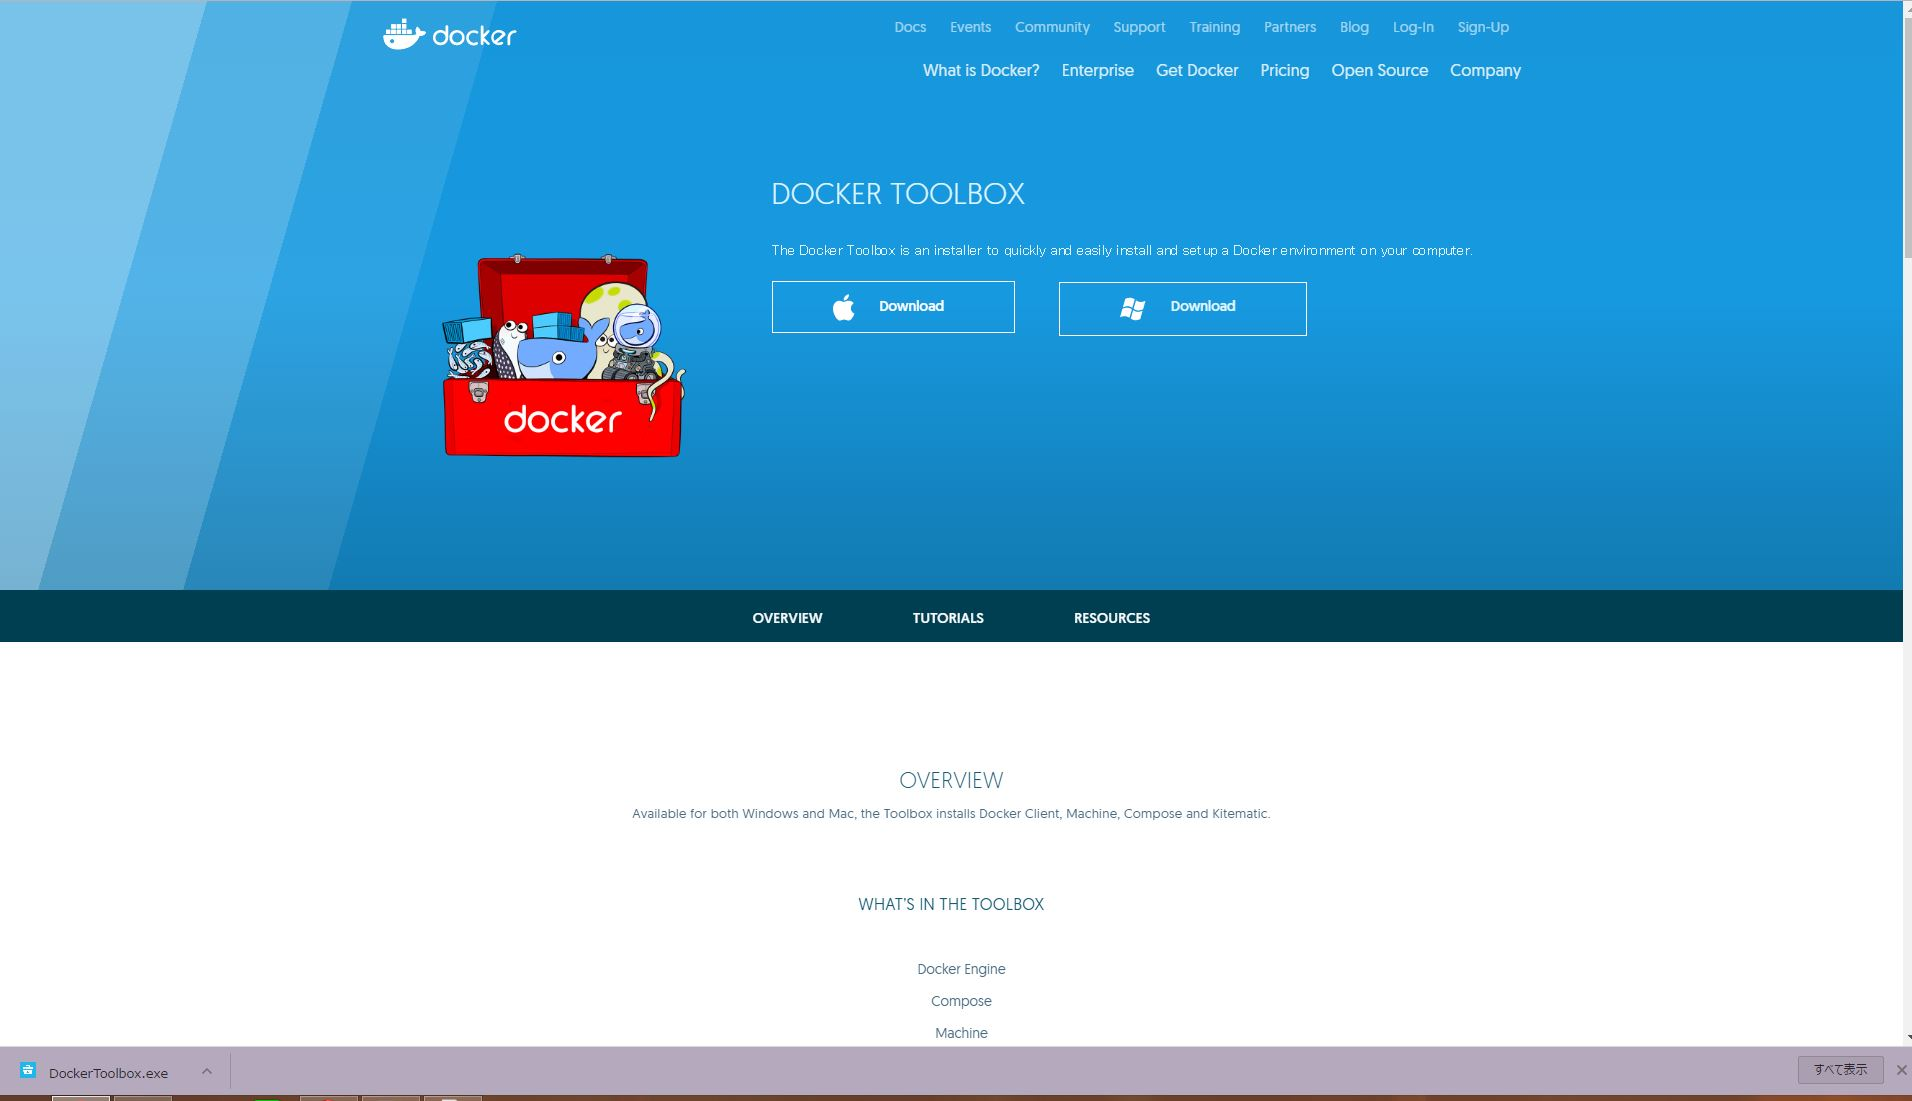
\includegraphics[width=11cm]{2.JPG}
\caption{Docker Toolboxのダウンロード}\label{tab:uac}
\end{figure}

Windows10以降は,Docker for Windowsをインストールできる.Windows10では,OSが提供するハイパーバイザ型の仮想マシンの上でDockerが利用できるようになった.それ以前は,Docker ToolboxによりVirtualBox上のLinuxにDockerEngineをインストールし,ホスト上のコマンドラインツールからアクセスするという手段を取る.
\newpage

\begin{figure}[htb]
\centering 
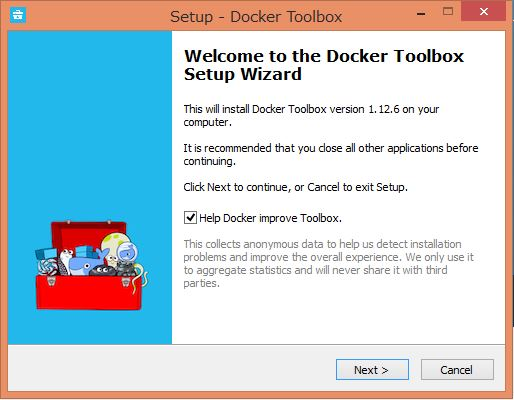
\includegraphics[width=11cm]{3.JPG}
\caption{セットアップウィザードの起動}\label{tab:uac}
\end{figure}

Nextを押す.

\newpage

\begin{figure}[htb]
\centering 
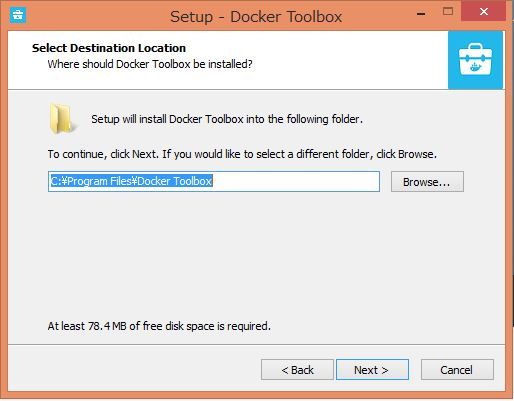
\includegraphics[width=11cm]{4.JPG}
\caption{インストールフォルダの選択}\label{tab:uac}
\end{figure}
Nextを押す.
\newpage

\begin{figure}[htb]
\centering 
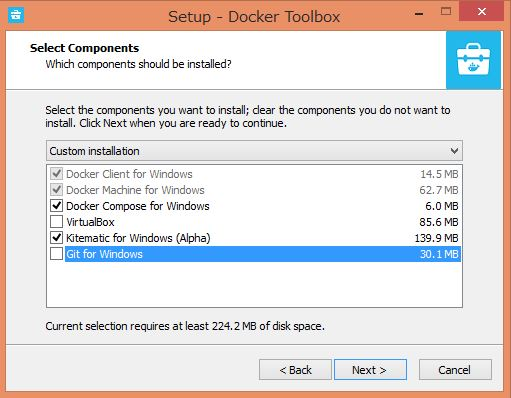
\includegraphics[width=11cm]{5.JPG}
\caption{インストールするコンポーネントの選択}\label{tab:uac}
\end{figure}
VirtualBoxとGit for Windowsを既にインストールしている場合はチェックを外す.インストールしていない場合はすべてチェックする.
\newpage

\begin{figure}[htb]
\centering 
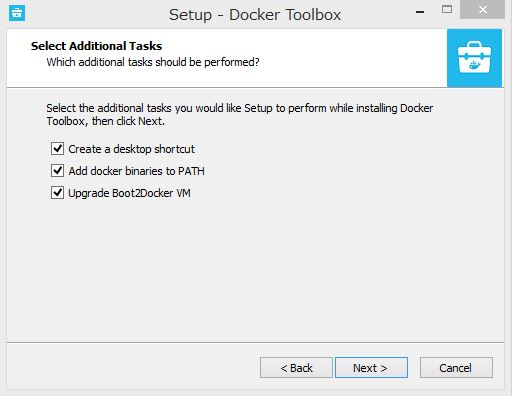
\includegraphics[width=11cm]{6.JPG}
\caption{インストール後の設定}\label{tab:uac}
\end{figure}
nextを押す.

\newpage



\begin{figure}[htb]
\centering 
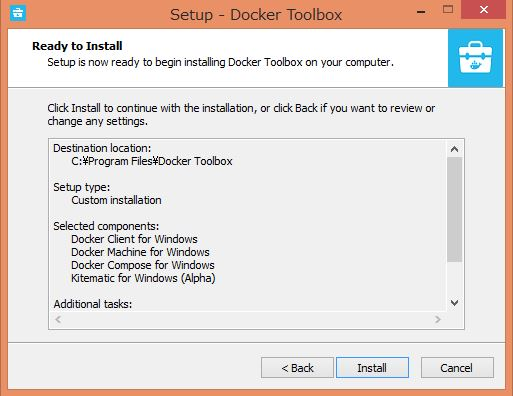
\includegraphics[width=11cm]{7.JPG}
\caption{インストール最終確認}\label{tab:uac}
\end{figure}
インストールが完了したらデスクトップに「Kitematic(Alpha)」と「Docker Quickstart Terminal」と「Oracle VM VirtualBox」の3つのアイコンが作成されます.まず,「Docker Quickstart Terminal」アイコンをダブルクリックしてください.
Docker ToolboxがDockerを動作させるための仮想環境を構築します.しばらく時間がかかりますが,処理が完了すると次のようなコンソール画面が表示される.
\newpage

\begin{figure}[htb]
\centering 
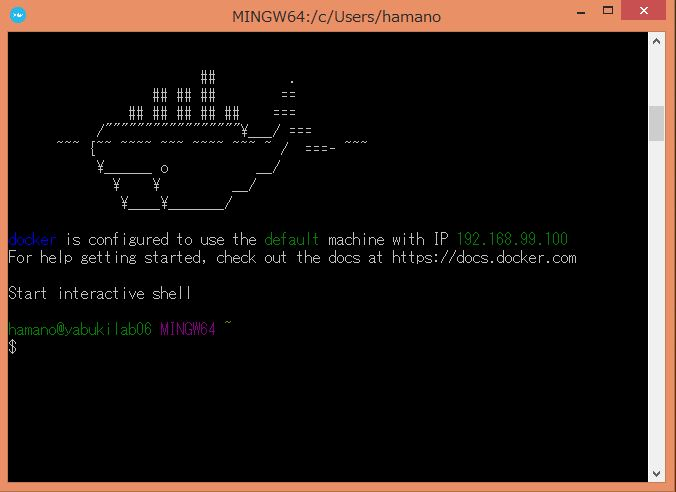
\includegraphics[width=11cm]{8.JPG}
\caption{Dockerの実行結果}\label{tab:uac}
\end{figure}
ログには,作成された仮想環境に割り当てられたマシン名(default)とIPアドレス(192.168.99.100)が表示される.
\newpage

以下コマンドにより,defaultという名前の仮想環境に対して,SSHで接続する.

\begin{lstlisting}[basicstyle=\ttfamily\footnotesize, frame=single]
$ docker-machine ssh default
\end{lstlisting}


\begin{figure}[htb]
\centering 
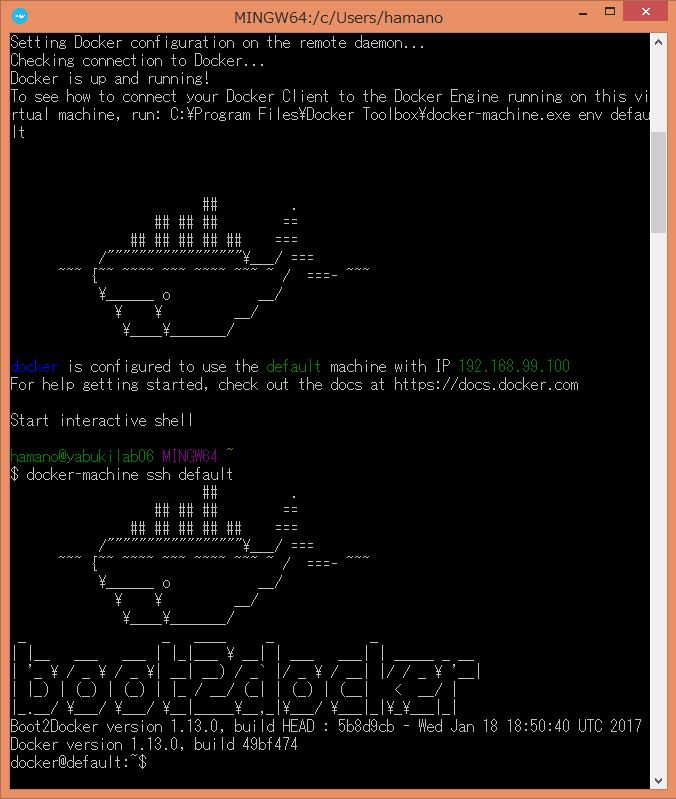
\includegraphics[width=11cm]{9.JPG}
\caption{仮想環境への接続}\label{tab:uac}
\end{figure}

以上でDocker環境が整った.

\newpage
\subsection{Dockerで「Hello world」}
インストールしたDockerが正しく動作するかを確認するため,Dockerコンテナを作成し,コンソール上に”Hello world”の文字をecho表示する.Dockerコンテナを作成/実行するときは,docker runコマンドを使う.
\begin{lstlisting}[basicstyle=\ttfamily\footnotesize, frame=single]
$ docker run ubuntu:latest /bin/echo `Hello world'
\end{lstlisting}

\begin{figure}[htb]
\centering 
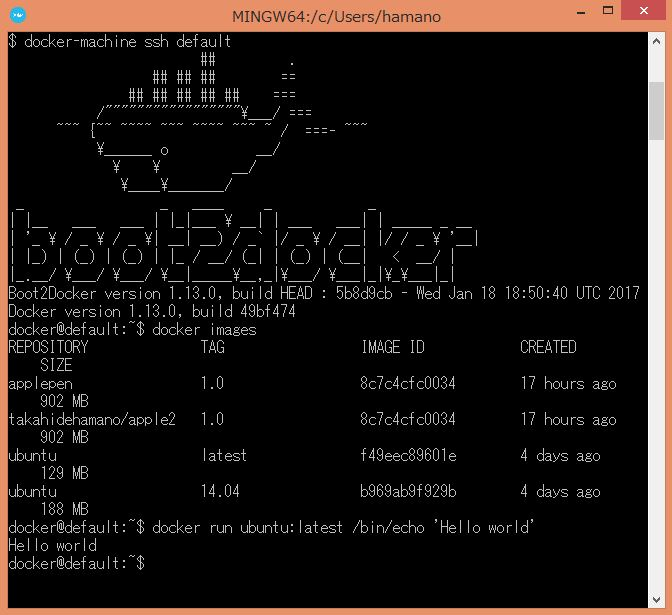
\includegraphics[width=11cm]{27.JPG}
\caption{Helloworldの実行結果}\label{tab:uac}
\end{figure}
\newpage
\subsection{ベースイメージの取得}
\begin{lstlisting}[basicstyle=\ttfamily\footnotesize, frame=single]
$ docker pull ubuntu
\end{lstlisting}
以下のコマンドで取得したイメージを確認する.
\begin{lstlisting}[basicstyle=\ttfamily\footnotesize, frame=single]
$ docker images
\end{lstlisting}
以下のような内容が出力される.
\begin{figure}[htb]
\centering 
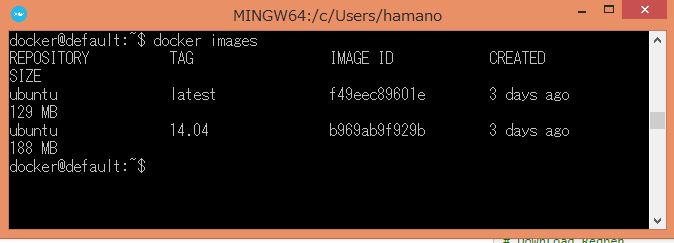
\includegraphics[width=14cm]{10.JPG}
\caption{docker images実行}\label{tab:uac}
\end{figure}

\newpage
\subsection{Dockerfile作成}
イメージを作成するためDockerfileを作成しビルドする.
Dockerfileは,Shell形式で記述する.

\begin{lstlisting}[basicstyle=\ttfamily\footnotesize, frame=single]
$ mkdir sample
$ cd sample

$ vi Dockerfile
\end{lstlisting}

Dockerfileは以下になる.
\begin{lstlisting}[basicstyle=\ttfamily\footnotesize, frame=single]
# Java 1.8 & RedPen Dockerfile
# https://github.com/kemsakurai/docker-redpen-UTF-8

# Pull base image.
FROM ubuntu:14.04

# maintainer details
MAINTAINER Ken Sakurai "sakurai.kem@gmail.com"

# Set locale
RUN locale-gen ja_JP.UTF-8
ENV LANG ja_JP.UTF-8
ENV LANGUAGE ja_JP:ja
ENV LC_ALL ja_JP.UTF-8

# Accecpt Oracle license before installing java
RUN echo debconf shared/accepted-oracle-license-v1-1 select true | debconf-set
-selections
RUN echo debconf shared/accepted-oracle-license-v1-1 seen true | debconf-set-s
elections

# Install java
RUN apt-get update
RUN apt-get -y install software-properties-common
RUN add-apt-repository -y ppa:webupd8team/java
RUN apt-get update
RUN apt-get -y install oracle-java8-installer oracle-java8-set-default
RUN echo "export JAVA_HOME=/usr/lib/jvm/java-8-oracle" >> /etc/environment

# DownLoad Redpen
WORKDIR /tmp
RUN wget -q https://github.com/redpen-cc/redpen/releases/download/redpen-1.5.5
/redpen-1.5.5.tar.gz -O - | tar xz && \
    cp -av redpen-distribution-1.5.5/* /usr/local/ && \
    rm -rf redpen-distribution-1.5.5

RUN export PATH=$PATH:/usr/local/bin
WORKDIR /data

CMD ["/usr/local/bin/redpen"]
\end{lstlisting}


\newpage
\subsection{DockerfileからDockerイメージの作成}

\begin{lstlisting}[basicstyle=\ttfamily\footnotesize, frame=single]
$ docker build -t applepen:1.0 .
\end{lstlisting}


docker imageコマンドによるイメージの確認
\begin{lstlisting}[basicstyle=\ttfamily\footnotesize, frame=single]
$ docker image
\end{lstlisting}
コマンドを実行すると以下のapplepenイメージが作成される.
\begin{figure}[htb]
\centering 
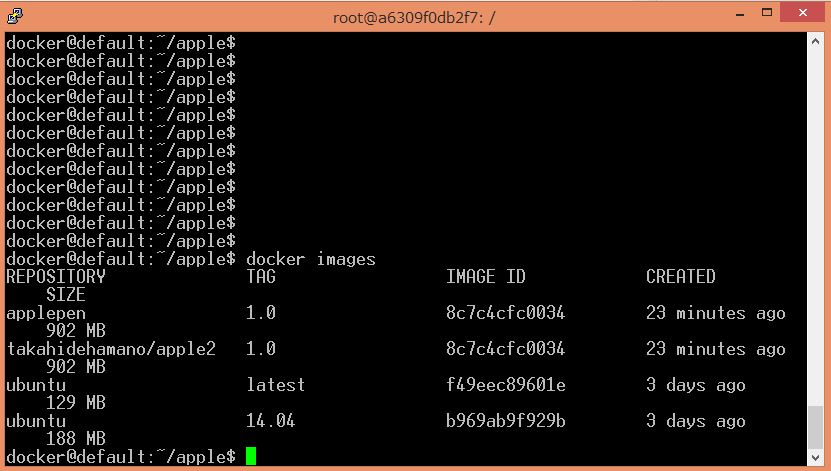
\includegraphics[width=11cm]{11.JPG}
\caption{docker imageコマンド実行}\label{tab:uac}
\end{figure}

\newpage 

\subsection{DockerHubログイン}
以下のコマンドを実行する.
\begin{lstlisting}[basicstyle=\ttfamily\footnotesize, frame=single]
$ docker login
Username:登録したユーザ名
Password:登録したパスワード
\end{lstlisting}
UsernameとPasswordを入力しログインする.



ログインに成功するとLogin Succededと表示される.

\newpage

\subsection{DockerHubにイメージをpush}
\begin{lstlisting}[basicstyle=\ttfamily\footnotesize, frame=single]
$ docker push takahidehamano/applepen:latest
\end{lstlisting}
DockerHubにログインし,リポジトリ一覧を確認する.Takahidehamano/applepenが作成されていることがわかる.
\begin{figure}[htb]
\centering 
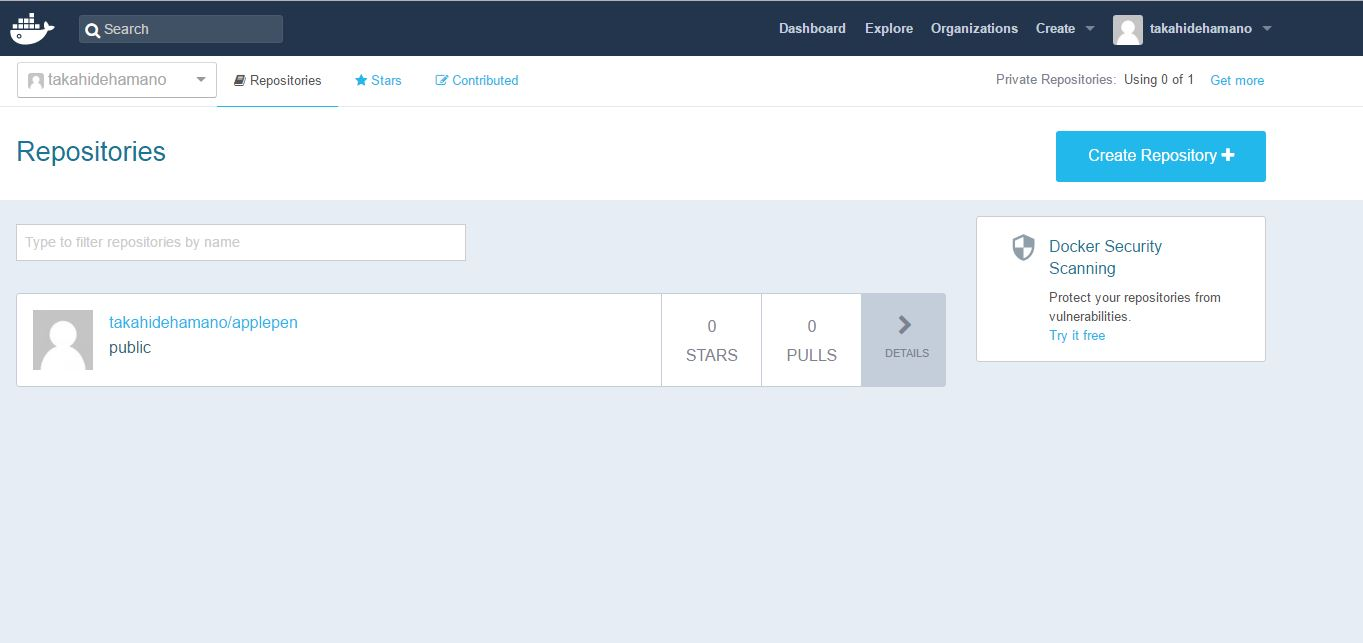
\includegraphics[width=11cm]{12.JPG}
\caption{DockerHub}\label{tab:uac}
\end{figure}

\chapter{自動化環境の構築}
\section{GitHubの設定}
\subsection{GitHubのリポジトリ}
GitHubのリポジトリを作成する.作成したリポジトリに文書をアップロードすることで文書チェックの自動化がされることが目的である.そのためWercker.ymlというWerckerを動かすためのコマンドが書かれたファイルとredpen-conf-ja.xmlという文書チェックプログラムRedPenの設定が書かれたファイルをGitHubリポジトリに用意する.
\begin{figure}[htb]
\centering 
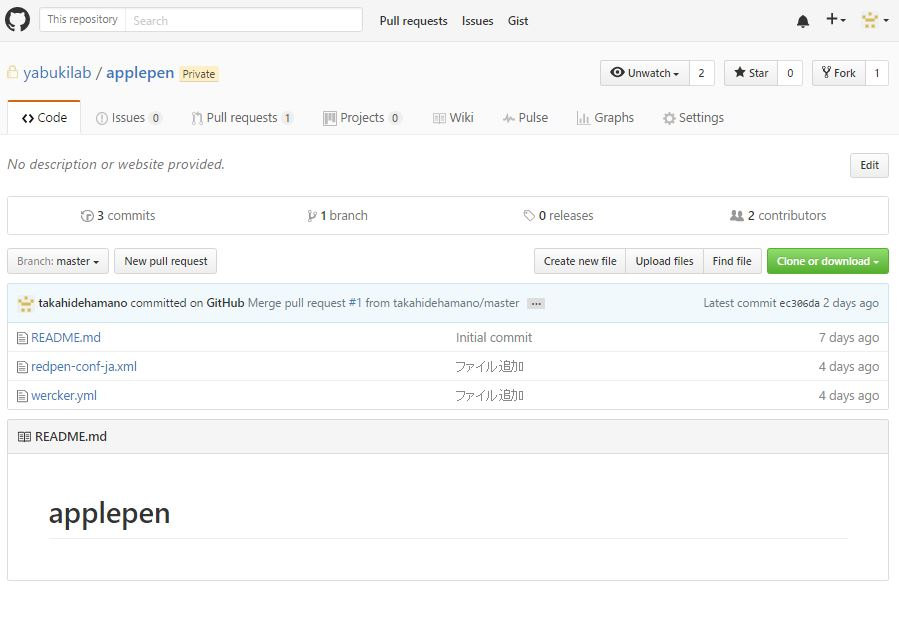
\includegraphics[width=11cm]{14.JPG}
\caption{GitHubリポジトリ}\label{tab:uac}
\end{figure}

\newpage
wercker.ymlの設定を以下に示す.
\begin{lstlisting}[basicstyle=\ttfamily\footnotesize, frame=single]
# This references a standard debian container from the
# Docker Hub https://registry.hub.docker.com/_/debian/
# Read more about containers on our dev center
# http://devcenter.wercker.com/docs/containers/index.html
box: takahidehamano/redpen
# You can also use services such as databases. Read more on our dev center:
# http://devcenter.wercker.com/docs/services/index.html
# services:
    # - postgres
    # http://devcenter.wercker.com/docs/services/postgresql.html

    # - mongodb
    # http://devcenter.wercker.com/docs/services/mongodb.html

# This is the build pipeline. Pipelines are the core of wercker
# Read more about pipelines on our dev center
# http://devcenter.wercker.com/docs/pipelines/index.html
build:
    # Steps make up the actions in your pipeline
    # Read more about steps on our dev center:
    # http://devcenter.wercker.com/docs/steps/index.html
  steps:
    - script:
        name: check
        code: |
        
          redpen -c ./redpen-conf-ja.xml -f latex  draft.tex

\end{lstlisting}
draft.texというtexの標準ファイルがリポジトリにpushされることでcheckというScriptが動作する仕組みになっている.
\newpage

redpen.conf-ja.xmlを以下に記述する.

\begin{lstlisting}[basicstyle=\ttfamily\footnotesize, frame=single]
<redpen-conf lang="ja" type="zenkaku2">
    <validators>
        <validator name="SentenceLength">
            <property name="max_len" value="100"/>
        </validator>
        <validator name="CommaNumber" />
        <validator name="SuccessiveWord" />
        <validator name="KatakanaSpellCheck"/>
        <validator name="InvalidExpression"/>
        <validator name="JapaneseStyle"/>
        <validator name="DoubleNegative" />
        <validator name="FrequentSentenceStart" />
        <validator name="JapaneseAmbiguousNounConjunction" />
        <validator name="JapaneseNumberExpression" />
        <validator name="SuccessiveSentence" />
        <validator name="DoubledConjunctiveParticleGa" />

        <validator name="DuplicatedSection" />
        <validator name="WordFrequency" />
        <validator name="ParenthesizedSentence" />

    </validators>
</redpen-conf>
\end{lstlisting}
RedPenが提供する設定を以下に示す.
\subsection{SentenceLength}
SentenceLength は入力文書に存在する各文(センテンス)の長さに関する規約が守られているかを検査します。 具体的には文書内の各文が指定された最大文長より長い場合、エラーを出力します。
\subsection{InvalidExpression}
入力に不正な表現(単語や句)が存在するか検査します。不正な表現が存在すると InvalidExpression はエラーを出力します。
\subsection{InvalidWord}
InvalidWord は入力文に不正な単語が存在するかを検査します。
\subsection{SpaceBeginningOfSentence}
SpaceBeginningOfSentence は文(センテンス)間に半角スペースが存在するかを検査します。
\subsection{CommaNumber}
CommaNumber は一文(センテンス)で利用されるコンマの数が指定された最大数よりも多いときにエラーを出力します。
\subsection{WordNumber}
WordNumber は一文内の単語数を検査します。文内の単語数が指定した数よりも大きいとき、WordNumber はエラー出力します。
\subsection{SuggestExpression}
SuggestExpression は InvalidExpression と同様に動作します。 入力文で不正な表現が使用されているとエラーを出力します。出力されるエラーには利用すべき正しい表現が含まれます。
\subsection{InvalidSymbol}
シンボルによっては代替のシンボルが存在します。 たとえばクエスチョンマーク ?(0x003F) は代替のシンボル ?(0xFF1F) が Unicode に登録されています。 InvalidSymbol は入力文で不正なシンボルが利用されているとエラーを出力します。


\subsection{SymbolWithSpace}
シンボルによっては前もしくは後にスペースが必要です。 たとえば、左括弧 "(" の前には、かならず半角スペースを置くという規約がありえます。 スペースに関する設定は設定ファイルの symbols ブロックで指定します。
\subsection{KatakanaEndHyphen}
カタカナ単語の語尾が規約(JIS Z8301 、G.6.2.2 b 、G.3.)に従っているかを検査します。 具体的には以下のルールが適用されます。

a: 単語が三文字もしくはそれ以上の場合には、ハイフンで単語は終わらない。

b: 単語が二文字もしくはそれ以下の場合には、単語はハイフンで終わってもよい。

c: 単語が複合語の場合には各々の部分単語について条件が適用される。

d: a から c のルールにおいて、拗音をのぞきハイフンは一文字としてカウントされます。
\subsection{KatakanaSpellCheck}
KatakanaSpellCheck はカタカナ単語のスペリングを検査します。 対象となるカタカナ単語に類似する単語が存在した場合、エラーを出力します。 たとえば、"インデックス"と"インデクス"が同一文書で利用されているときにエラーを出力します。
\subsection{SectionLength}
SectionLength は節で利用できる単語の数を指定します。
\subsection{ParagraphNumber}
ParagraphNumber は節の中に存在してよいパラグラフの最大数を指定します。

\subsection{ParagraphStartWith}
ParagraphStartWith はパラグラフの開始部分が指定された規約に従っているかを検査します。
\subsection{SpaceBetweenAlphabeticalWord}
アルファベット単語の前後に空白が存在するかを検査します。 単語が空白によって区切られない言語(日本語、中国語など)で執筆するときに使用します。 SpaceBetweenAlphabeticalWord はアルファベット単語の前後に空白が存在しないとエラーを出力します。
\subsection{DoubledWord}
DoubledWord は一文内で二回以上、同一の単語が使用されたときにエラーを出力します。 たとえば、以下の文では良いが二回使われているので、エラーを出力します。
\subsection{SuccessiveWord}
SuccessiveWord は同一の単語が連続して使用されたときにエラーを出力します。

たとえば入力文書に以下の文が含まれていると、エラーを出力します。 以下の文は、言語という単語を連続(書き誤り)で使用しています。
\subsection{DuplicatedSection}
文書中に著しく類似する節が存在すると、エラーを出力します。 類似度はコサイン距離によって計算されます。
\subsection{JapaneseStyle}
ですます調とである調が混在して利用された場合、エラーを出力します。
\subsection{DoubleNegative}
DoubleNegative は入力文書に二重否定が使用されているとエラーを出力します。
\subsection{FrequentSentenceStart}
多くの文が同一表現から開始されているときにエラーを出力します。
\subsection{ParenthesizedSentence}
ParenthesizedSentence は括弧に関する規約を検査します。 検査するポイントは以下の3つです。

一文内で使用される括弧の使用頻度

ネストされた括弧が存在するか

括弧の開始位置から終了位置までの長さ
\subsection{JavaScript}
JavaScript は機能拡張スクリプトを実行します。
\subsection{DoubledJoshi}
DoubledJoshi は同一の助詞が一文で二回以上、利用されているとエラーを出力します。
\subsection{HankakuKana}
文書中に半角カナ文字が利用されているとエラーを出力します。
\subsection{Okurigana}
送りがなの使い方が正しくない場合にエラーを出力します。
\subsection{VoidSection}
節に段落や文が1つも含まれていない場合にエラーを出力します。
\subsection{GappedSection}
GappedSection は節(章)の大きさにギャップがあるとエラーを出力します。 たとえば、以下のテキストでは 1 節の直下に 1.1.1 節があります。 つまり 1 節と 1.1.1 節の間にギャップが存在します。 ギャップを埋めるためには、1.1.1 節の前に 1.1 節が存在するべきです。
\subsection{LongKanjiChain}
長すぎる熟語(漢字の連続)を検出し、エラーを出力します。
\subsection{SectionLevel}
深すぎる節を検出しエラーを出力します。
\subsection{JapaneseAmbiguousNounConjunction}
日本語文に含まれる、曖昧な名詞接続のパターンを検出しエラーを出力します。 ここで、曖昧な名詞接続のパターンとは、格助詞の "の" + 名詞連続 + 各助詞の "の" です。 たとえば以下の文は、曖昧な名詞接続を含んでいます。
\subsection{JapaneseAnchorExpression}
日本語文において、章節の参照が一貫したスタイルになっているか検査します。
\subsection{SuccessiveSentence}
SuccessiveSentence は同一の文が二回連続で使用されるとエラーを出力します。

たとえば入力文書に以下のパラグラフが含まれていると、エラーを出力します。

いつも感じるのです。日本語はよい言語だ。日本語はよい言語だ。それでも別の言語もよい点が色々あります。
上記のパラグラフには同一の文 "日本語はよい言語だ。" が二回連続で出現しています。
\subsection{DoubledConjunctiveParticleGa}
一文に二回以上、接続助詞の が が出現するとエラーを出力します。たとえば、DoubledConjunctiveParticleGa は以下の文に対してエラーを出力します。


\newpage
\section{Werckerの設定}
http://www.wercker.com/
\begin{figure}[htb]
\centering 
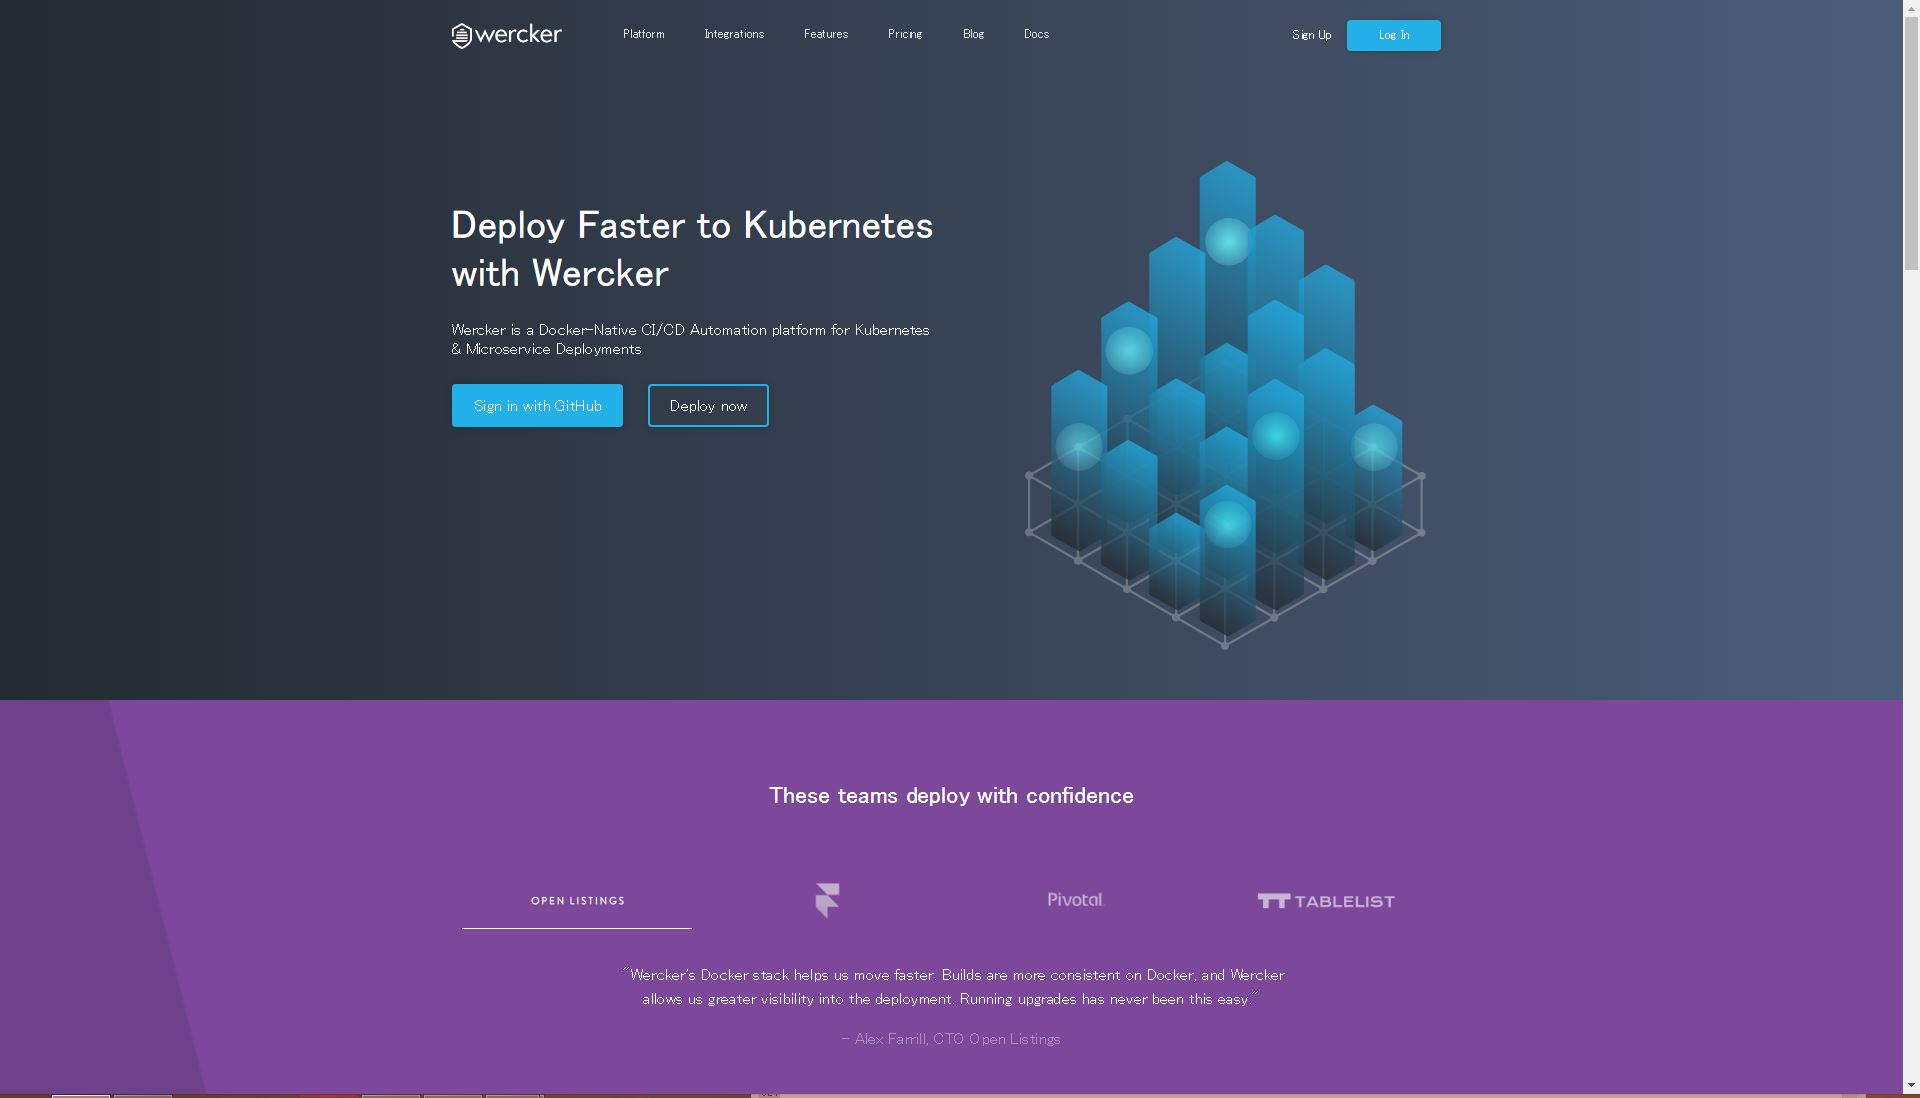
\includegraphics[width=11cm]{13.JPG}
\caption{自動化ツールWerckerとGitHubの連携}\label{tab:uac}
\end{figure}
GitHubのアカウントを用いログインする.

\newpage

上のタブのCreateからAppricationをクリックする.

\begin{figure}[htb]
\centering 
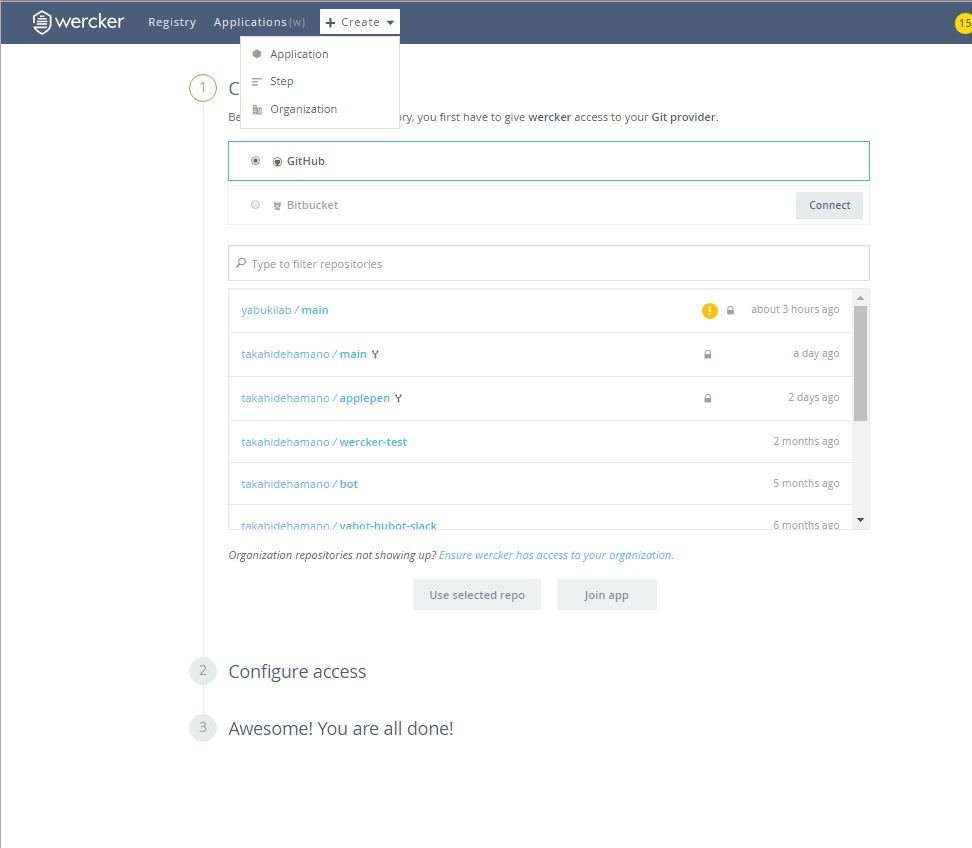
\includegraphics[width=11cm]{15.JPG}
\caption{Wercker Create}\label{tab:uac}
\end{figure}
GitHubを選択し,表示されているリポジトリの中からtakahidehamano/applepenを選択する.
\newpage
\begin{figure}[htb]
\centering 
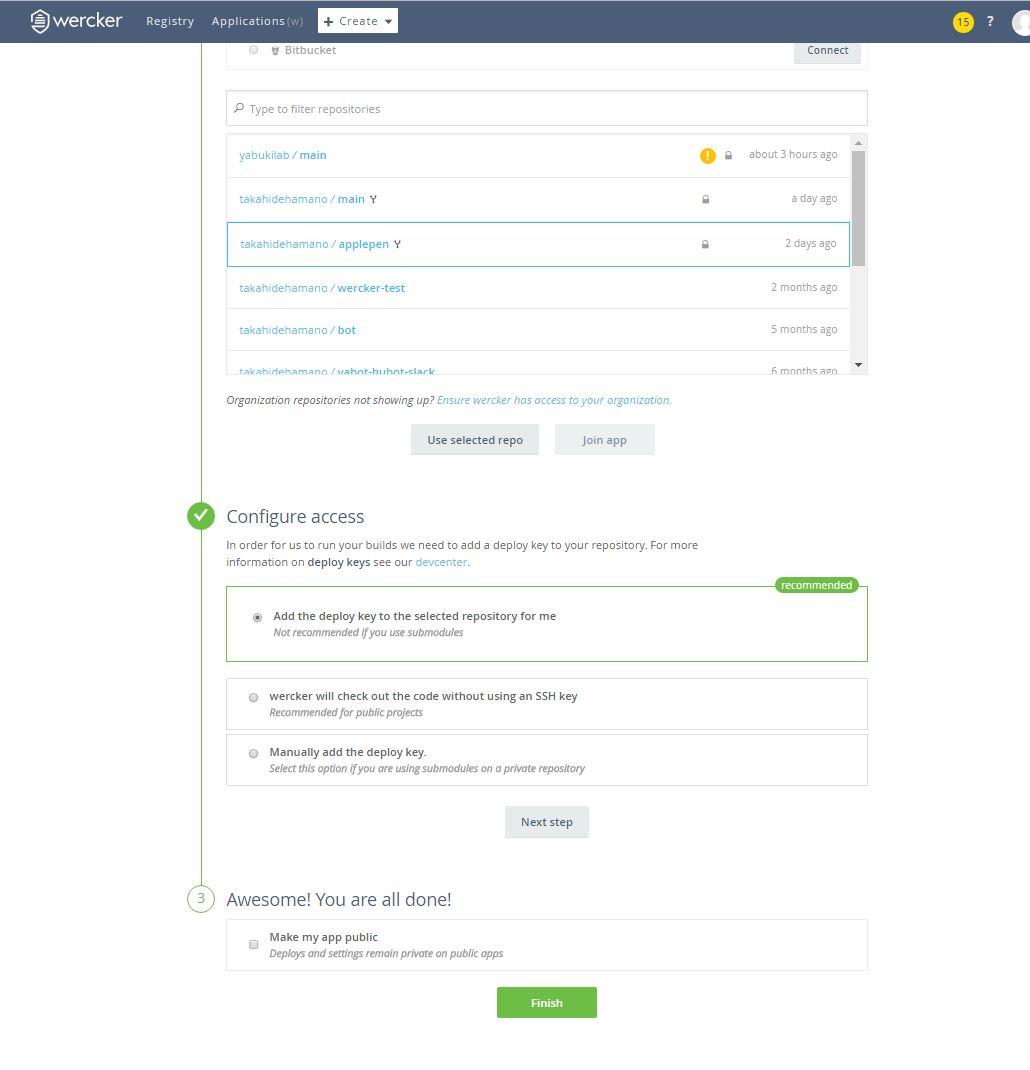
\includegraphics[width=11cm]{16.JPG}
\caption{Wercker Create}\label{tab:uac}
\end{figure}
Finishボタンを押すことでWerckerアプリケーションが構築される.

\newpage
\begin{figure}[htb]
\centering 
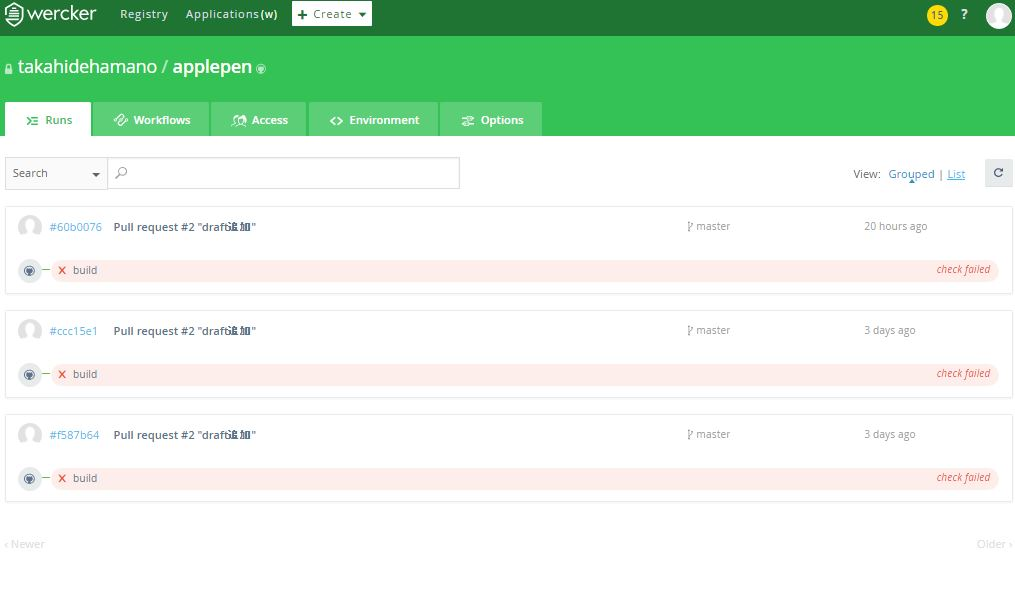
\includegraphics[width=11cm]{35.JPG}
\caption{Werckerアプリケーション完成}\label{tab:uac}
\end{figure}


\chapter{GitHubに文書提出}
GitHubリポジトリをForkする.
以下の画面の右上にForkボタンがある.
\begin{figure}
\centering 
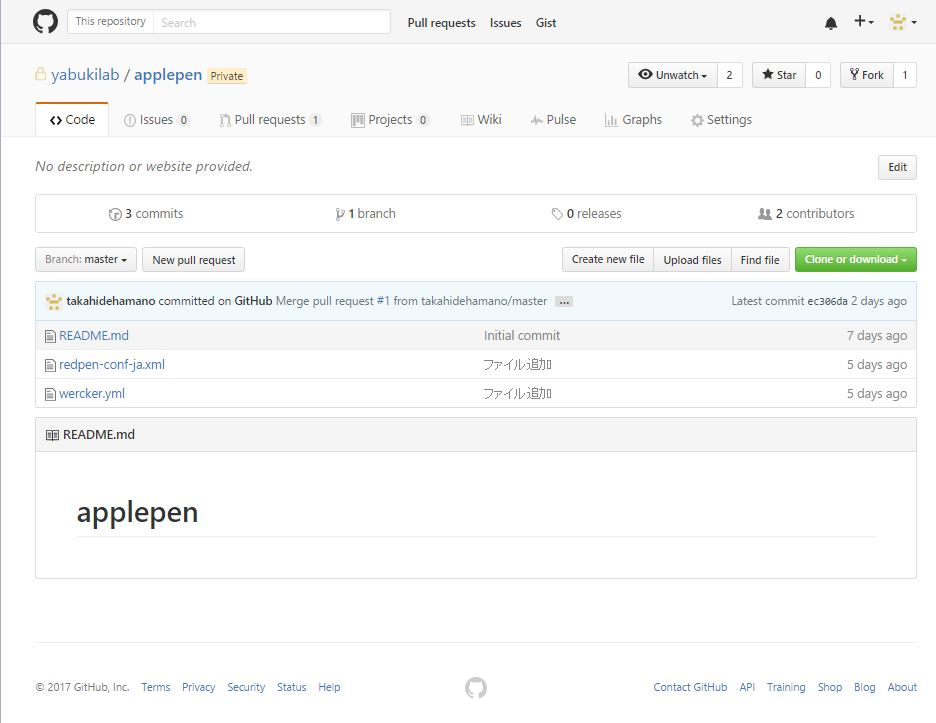
\includegraphics[width=11cm]{17.JPG}
\caption{GitHubリポジトリ}\label{tab:uac}
\end{figure}
\newpage
次にClone of downloadを押す.ボタンは真ん中の右側にある.
\begin{figure}[htb]
\centering 
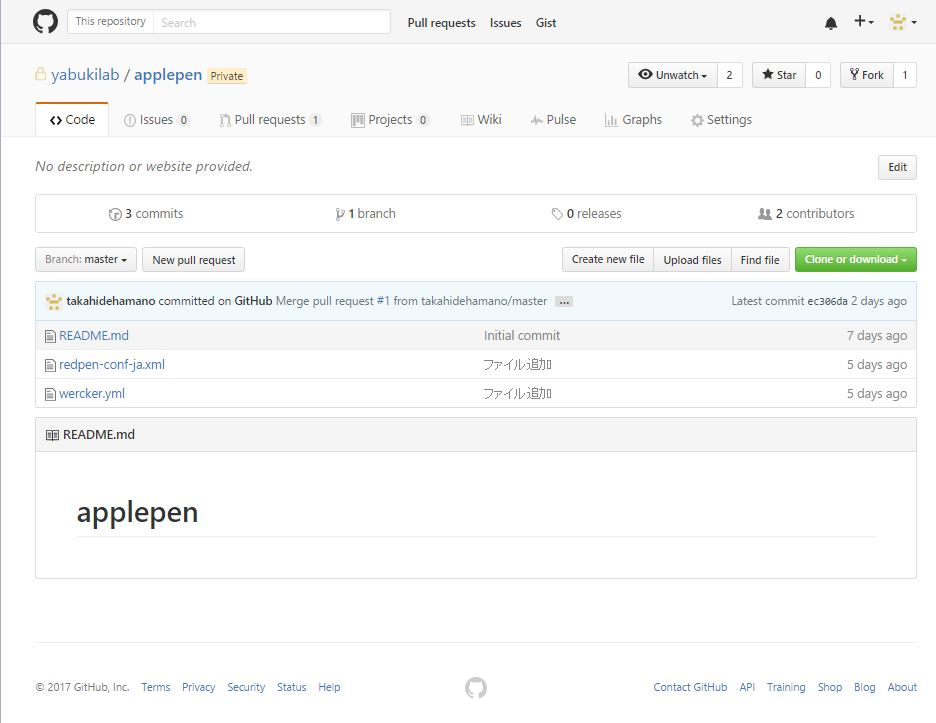
\includegraphics[width=11cm]{17.JPG}
\caption{GitHubリポジトリ}\label{tab:uac}
\end{figure}
\newpage
GitHubアプリケーションにapplepenがcloneされる.
\begin{figure}
\centering 
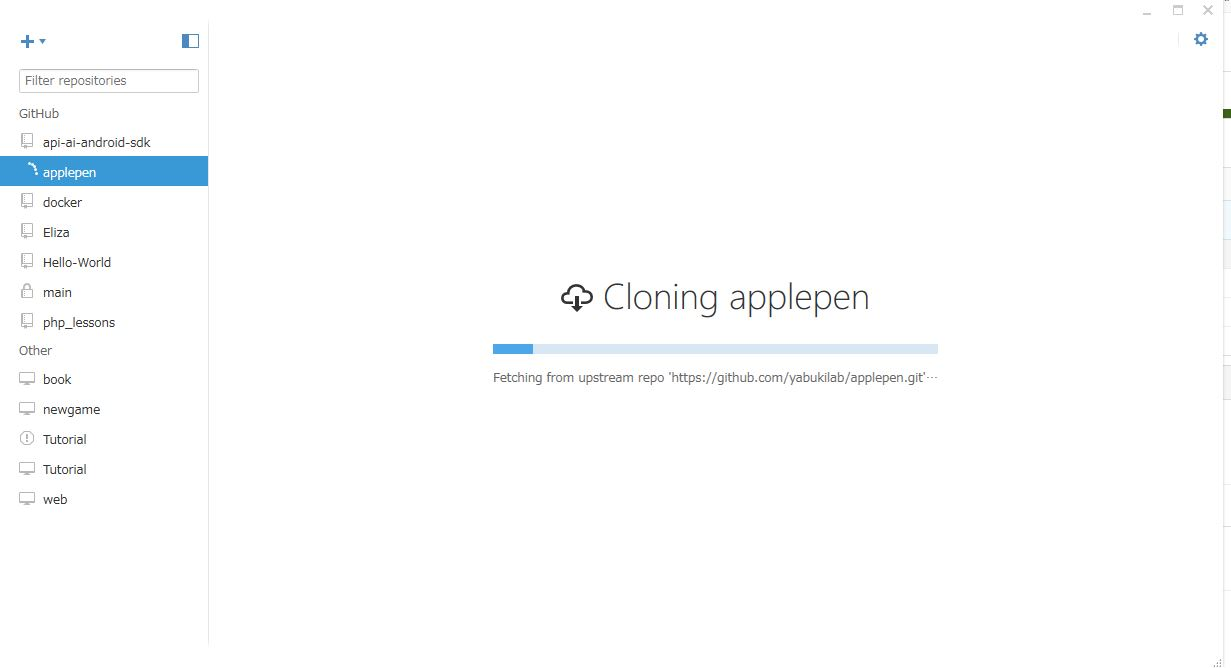
\includegraphics[width=11cm]{19.JPG}
\caption{GitHub Clone}\label{tab:uac}
\end{figure}
\newpage
ローカルにapplepenリポジトリのファイルが保存される.
\begin{figure}
\centering 
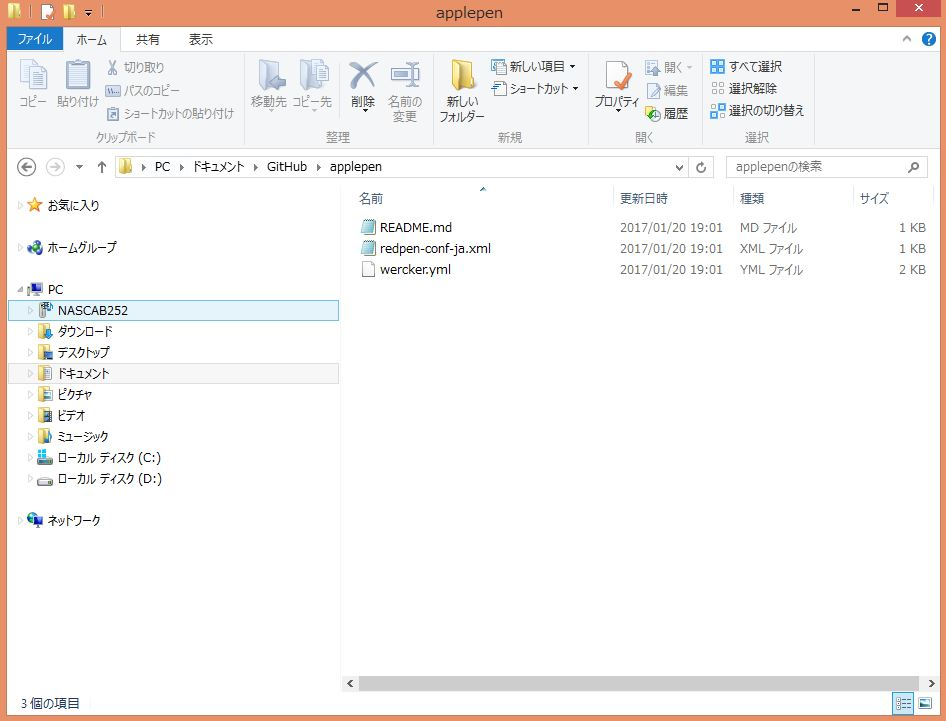
\includegraphics[width=11cm]{18.JPG}
\caption{ローカルリポジトリ}\label{tab:uac}
\end{figure}
\newpage

ローカルに保存されたファイルの中にTeXファイルを保存する.

\begin{figure}
\centering 
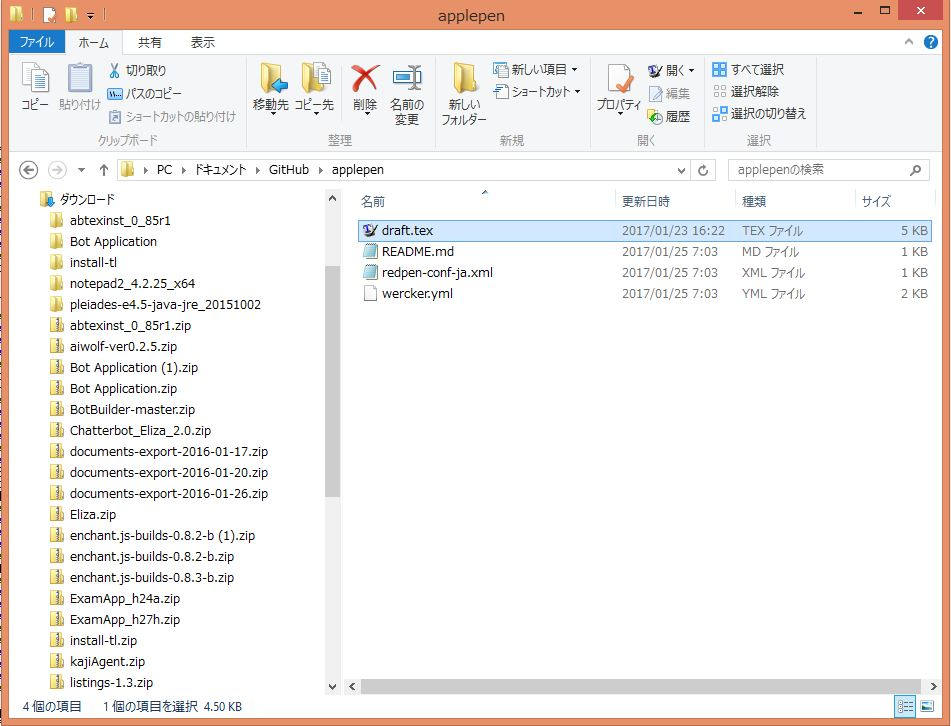
\includegraphics[width=11cm]{21.JPG}
\caption{drafte.tex追加}\label{tab:uac}
\end{figure}
\newpage

GitHubアプリケーションを開く
\begin{figure}
\centering 
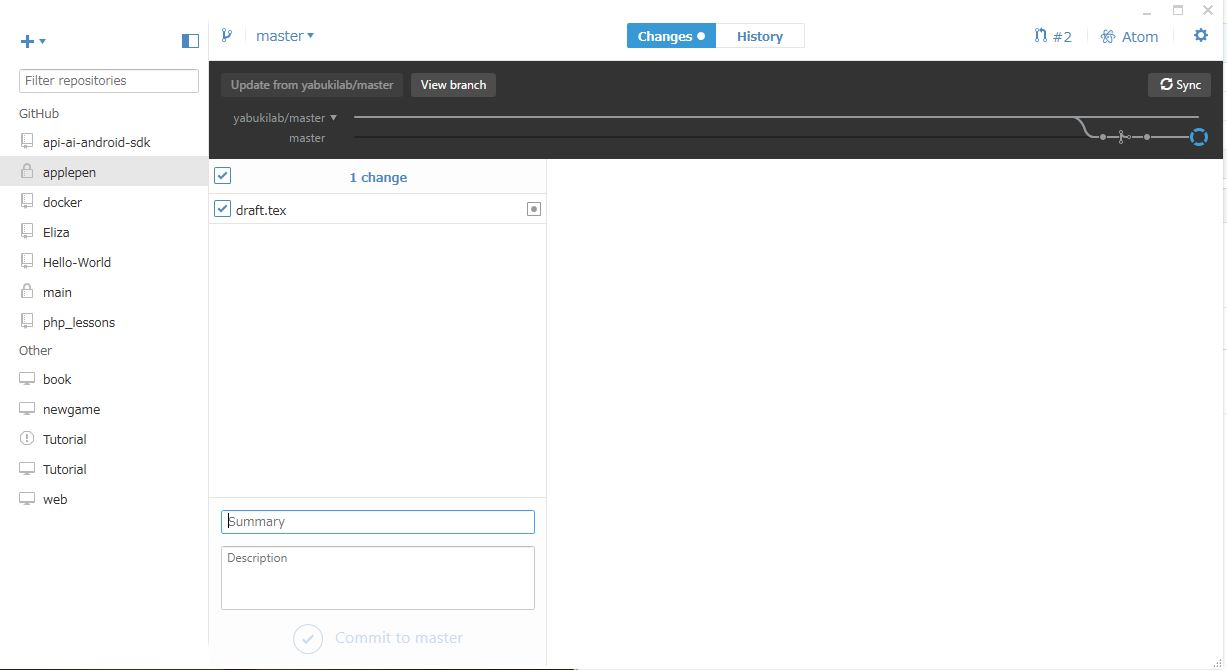
\includegraphics[width=11cm]{20.JPG}
\caption{GitHubアプリケーション}\label{tab:uac}
\end{figure}

\newpage

先のローカルリポジトリの変更をコメントをつけてCommitする.
\begin{figure}
\centering 
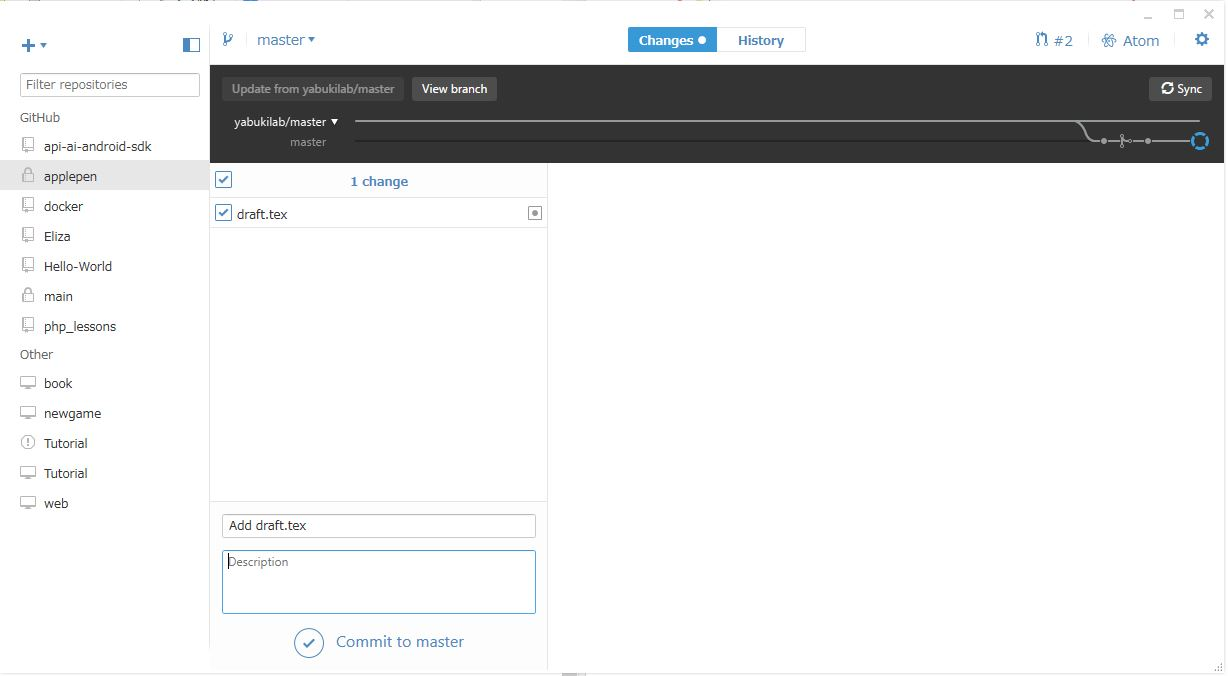
\includegraphics[width=11cm]{22.JPG}
\caption{Commit}\label{tab:uac}
\end{figure}

\newpage

Syncを行う.画面の右上にボタンがある.
\begin{figure}
\centering 
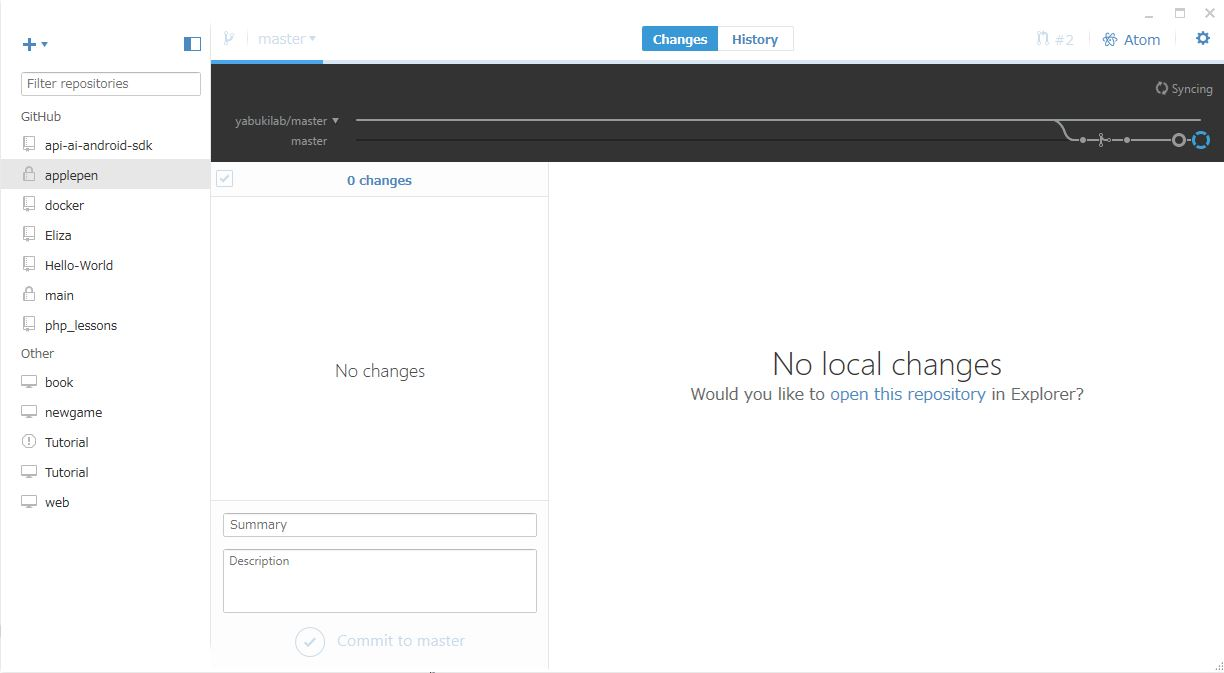
\includegraphics[width=11cm]{23.JPG}
\caption{Sync}\label{tab:uac}
\end{figure}

\newpage
最初のリポジトリの画面からFork前のリポジトリに移る.
\begin{figure}
\centering 
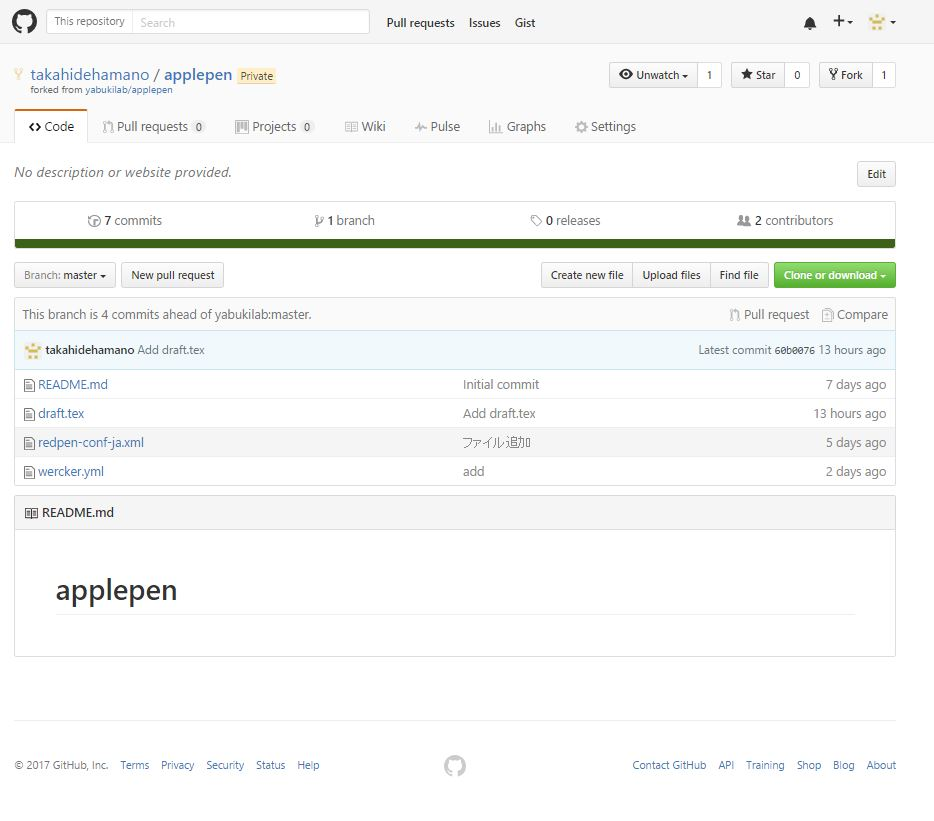
\includegraphics[width=11cm]{31.JPG}
\caption{PullRequest}\label{tab:uac}
\end{figure}
\newpage
PullRequestタブを開きNewPullRequestを行う.
そうすることでwerckerが立ち上がり自動で文書チェックプログラムが起動する.
文章チェックプログラムの結果の表示にはDetailsを押す.
\begin{figure}
\centering 
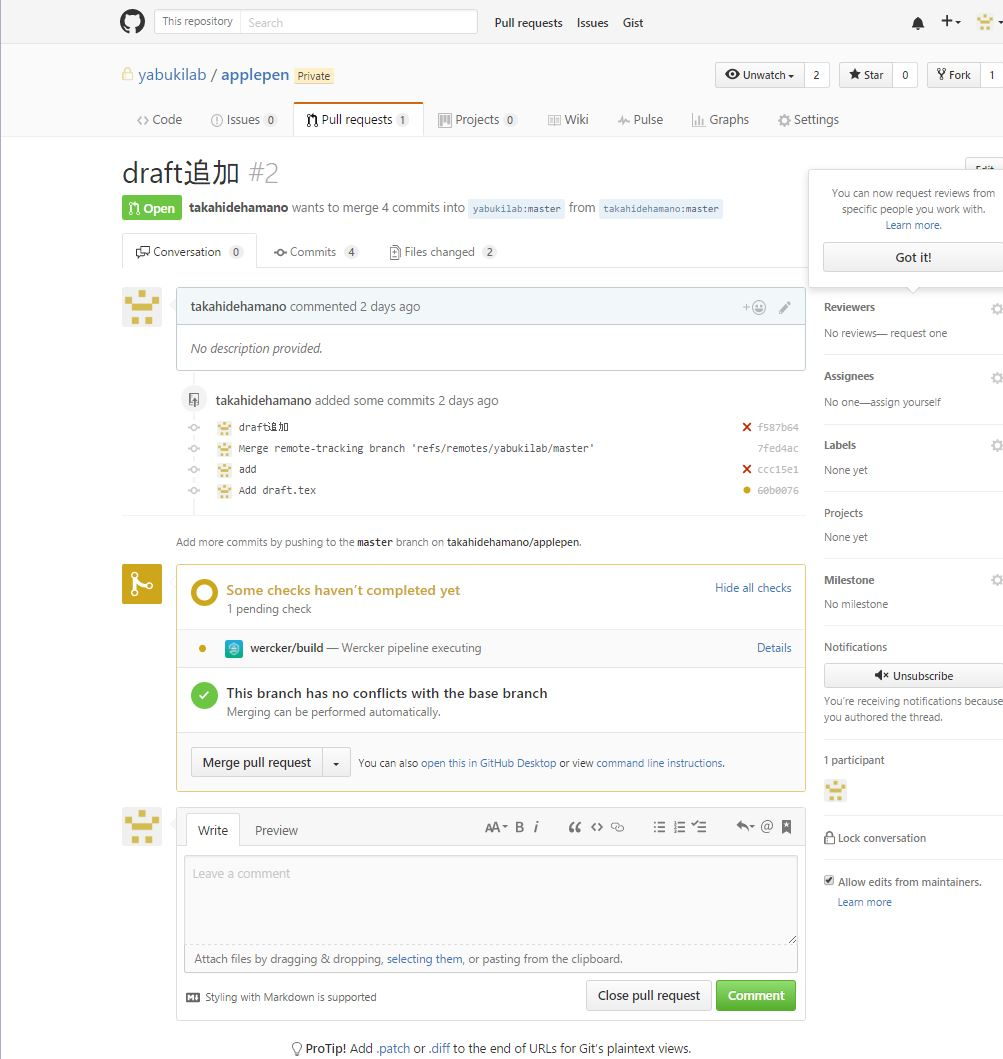
\includegraphics[width=11cm]{24.JPG}
\caption{PullRequest}\label{tab:uac}
\end{figure}

\newpage
文章チェック結果を表示する.
\begin{figure}
\centering 
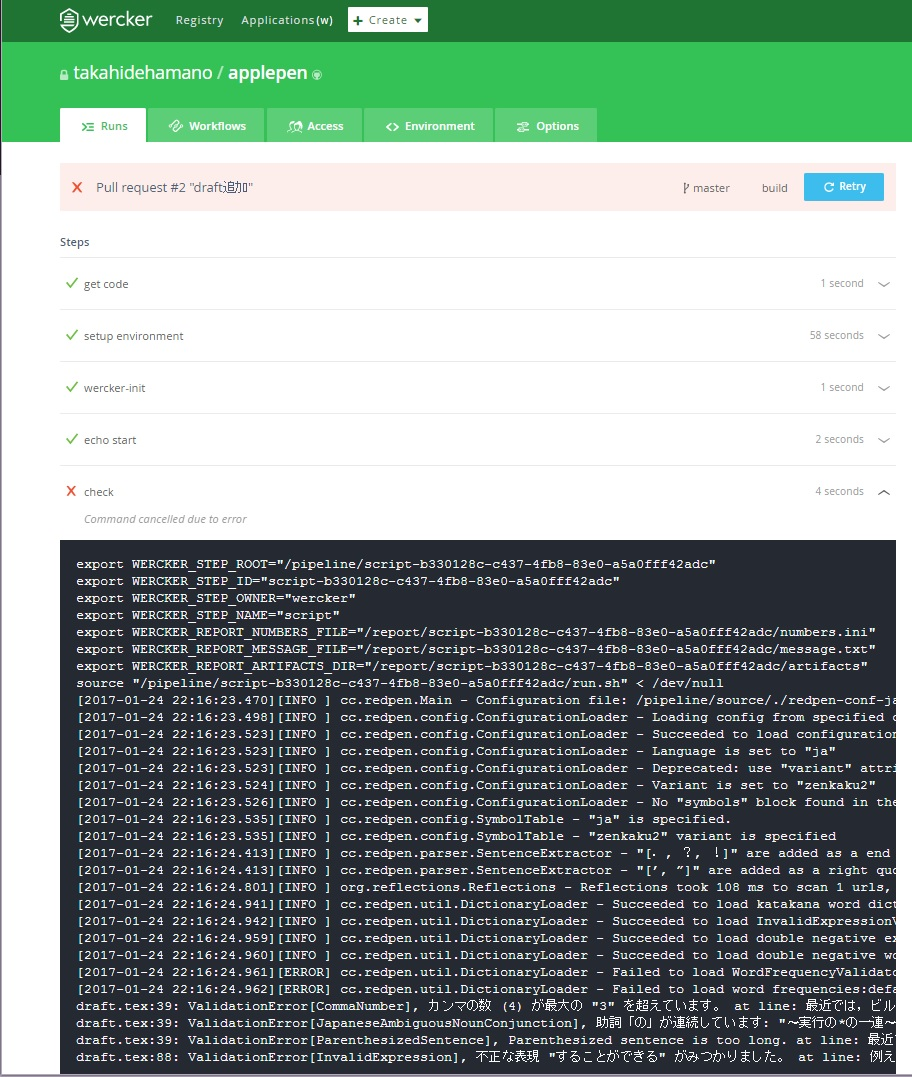
\includegraphics[width=11cm]{25.JPG}
\caption{Wercker}\label{tab:uac}
\end{figure}
\chapter{結果}
GitHubに課題研究の概要を提出した場合,文章チェックプログラムによって自動的に文章チェックが行えるようになった.
課題研究の概要を文書チェックにかけてみたところ以下の指摘が表示された.
\begin{enumerate}
\item SentenceLength - 文長を検査する.
\item InvalidExpression - 不正な表現が利用されていないか検査する.
\item KatakanaSpellCheck - カタカナ単語のスペルチェックを行う.
\item JapaneseAmbiguousNounConjunction - 助詞の「の」が連続しているか検査する.
\end{enumerate}
\begin{figure}[htb]
\centering 
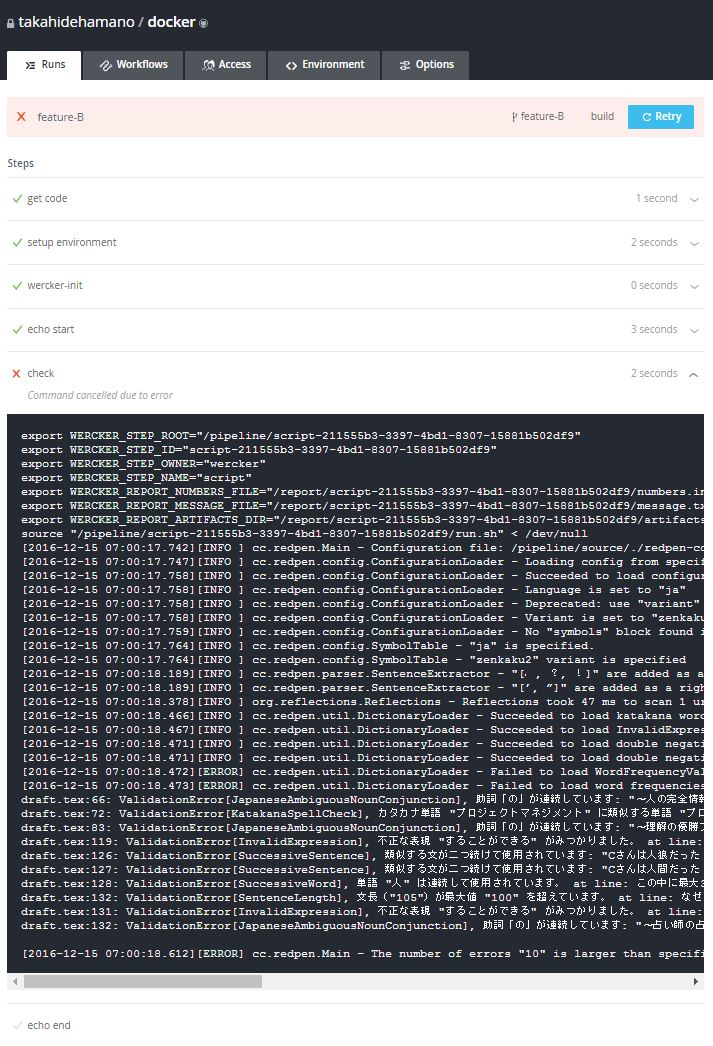
\includegraphics[width=11cm]{34.JPG}
\caption{文書チェック結果}
\end{figure}

\chapter{考察}
文書チェックプログラムは設定ファイルを変更することで,出力結果も変わる.そのため設定を変更し,添削に有効な設定を検討する必要がある.例えば添削前の文書を文書チェックプログラムにかけ,どの範囲まで文書の誤りをチェックすることができるのか調べることで,文書チェックプログラムが添削できる範囲を調べることができると考えた.
\chapter{結論}

自動的に文書チェックを行う環境を構築することができた.文書チェックプログラムの設定に関しては詳しく調べることができなかったため,検証が必要である.





\bibliographystyle{junsrt}
\bibliography{biblio}%「biblio.bib」というファイルが必要.



\end{document}
